\chapter{Elements}
\label{c:elements}
\index{element|hyperbf}

A lattice is made up of a collection of elements --- quadrupoles,
bends, etc. This chapter discusses the various classes of elements
available in \bmad except for \vn{group}s and \vn{overlay}s which are
discussed \cref{c:control}

\index{MAD}
Most element classes available in \mad are provided in \bmad.
Additionally, \bmad provides a number of element classes that are not
available in \mad.  A word of caution: In some cases where both \mad
and \bmad provide the same element class, there will be an overlap of
the attributes available but the two sets of attributes will not be
the same.  The list of element classes known to \bmad is shown in
Table~\ref{t:particle.classes}, \ref{t:photon.classes}, and
\ref{t:control.classes}.  Table~\ref{t:particle.classes} lists the
elements suitable for use with relativistic particles,
Table~\ref{t:photon.classes} which lists the elements suitable for use
with photons, and finally Table~\ref{t:control.classes} lists the
element classes that can be used for parameter control of other
elements.  Note that some classes are suitable for both particle and
photon use.

\begin{table}[ht]
\centering
{\tt
\begin{tabular}{|l|l||l|l|} \hline
  {\it Element}     & {\it Section}       & {\it Element}    & {\it Section}    \HH
  AB_Multipole      & \ref{s:ab.m}        &  Null_Ele        & \ref{s:null.ele} \HH
  BeamBeam          & \ref{s:bbi}         &  Octupole        & \ref{s:oct}      \HH
  Bend_Sol_Quad     & \ref{s:bsq}         &  Patch           & \ref{s:patch}    \HH
  Branch            & \ref{s:branch}      &  Photon_Branch   & \ref{s:branch}   \HH
  Custom            & \ref{s:custom}      &  Pipe            & \ref{s:monitor}  \HH
  Drift             & \ref{s:drift}       &  Quadrupole      & \ref{s:quad}     \HH
  Ecollimator       & \ref{s:col}         &  Rbend           & \ref{s:bend}     \HH
  ElSeparator       & \ref{s:elsep}       &  Rcollimator     & \ref{s:col}      \HH
  HKicker           & \ref{s:hvkicker}    &  RFcavity        & \ref{s:rfcav}    \HH
  Hybrid            & \ref{s:hybrid}      &  Sbend           & \ref{s:bend}     \HH
  Instrument        & \ref{s:monitor}     &  Sextupole       & \ref{s:sex}      \HH
  Kicker            & \ref{s:kicker}      &  Solenoid        & \ref{s:sol}      \HH
  Lcavity           & \ref{s:lcav}        &  Sol_Quad        & \ref{s:sq}       \HH
  Marker            & \ref{s:mark}        &  Taylor          & \ref{s:tay}      \HH
  Match             & \ref{s:match}       &  VKicker         & \ref{s:hvkicker} \HH  
  Monitor           & \ref{s:monitor}     &  Wiggler         & \ref{s:wiggler}  \HH
  Multipole         & \ref{s:mult}        &                  &                  \HH

\end{tabular}
}
\caption{Table of element classes suitable for use with relativistic particles.}
\label{t:particle.classes}\center
\end{table}

\begin{table}[ht]
\centering
{\tt
\begin{tabular}{|l|l||l|l|} \hline
  {\it Element}      & {\it Section}         & {\it Element}      & {\it Section}      \HH
  Capillary          & \ref{s:capillary}     &  Match             & \ref{s:match}      \HH
  Crystal            & \ref{s:crystal}       &  Monitor           & \ref{s:monitor}    \HH 
  Custom             & \ref{s:custom}        &  Mirror            & \ref{s:mirror}     \HH
  Drift              & \ref{s:drift}         &  Multilayer_mirror & \ref{s:multilayer} \HH
  Instrument         & \ref{s:monitor}       &  Patch             & \ref{s:patch}      \HH
  Marker             & \ref{s:mark}          &  Pipe              & \ref{s:monitor}    \HH
\end{tabular}
}
\caption{Table of element classes suitable for use with photons.}
\label{t:photon.classes}\center
\end{table}

\begin{table}[ht]
\centering
{\tt
\begin{tabular}{|l|l||l|l|} \hline
  {\it Element}  & {\it Section}     & {\it Element}  & {\it Section}    \HH
  Group          & \ref{s:group}     &   Overlay      & \ref{s:overlay}  \HH
  Girder         & \ref{s:girder}    &                &                  \HH
\end{tabular}
}
\caption{Table of element classes used for parameter control of other elements.}
\label{t:control.classes}\center
\end{table}

%-----------------------------------------------------------------
\section{AB_Multipole}
\label{s:ab.m}
\index{ab_multipole|hyperbf}

An \vn{ab_multipole} is a thin multipole lens up to 20th order. The
basic difference between this and a \vn{multipole} (\sref{s:mult} is
the input format. See section~\sref{s:fields} for how the multipole
coefficients are defined.

General \vn{ab_multipole} Attributes are:
\begin{center}
\tt 
\begin{tabular}{|l|l||l|l|} \hline
  {\sl Attribute Class}  & \s              & {\sl Attribute Class}      & \s              \HH
  a$n$, b$n$ multipoles  & \ref{s:multip}  & Offsets and tilt           & \ref{s:offset}  \HH
  Description strings    & \ref{s:string}  & Is_on                      & \ref{s:is.on}   \HH 
  Reference energy       & \ref{s:energy}  & Tracking \& transfer map   & \ref{c:methods} \HH
  Aperture Limits        & \ref{s:limit}   & Length                     & \ref{s:l}       \HH
\end{tabular}
\end{center}
\toffset

For \vn{a$n$} and \vn{b$n$}, $n$ is in the range 0 through 20.

\index{x_pitch}\index{y_pitch}
The length \vn{l} is a fictitious length that is used for synchrotron
radiation computations and affects the longitudinal position of the
next element but does not affect any tracking or transfer map
calculations.  The \vn{x_pitch} and \vn{y_pitch} attributes are not
used in tracking.

Like a \mad \vn{multipole}, an \vn{ab_multipole} will affect the
reference orbit if there is a dipole component. 

Example:
\begin{example}
  abc: ab_multipole, a2 = 0.034e-2, b3 = 5.7, a11 = 5.6e6/2
\end{example}

%-----------------------------------------------------------------
\section{BeamBeam}
\label{s:bbi}
\index{beambeam|hyperbf}

A \vn{beambeam} element simulates an interaction with an opposing
(``strong'') beam traveling in the opposite direction. The strong beam
is assumed to be Gaussian in shape. In the \vn{bmad_standard}
calculation the beam--beam kick is computed using the
Bassetti--Erskine complex error function formula\cite{b:talman}

General \vn{beambeam} attributes are:
\begin{center} 
\tt
\begin{tabular}{|l|l||l|l|} \hline
  {\sl Attribute Class}  & \s              & {\sl Attribute Class}      & \s              \HH
  Aperture Limits        & \ref{s:limit}   & Offsets, pitches, and tilt & \ref{s:offset}  \HH
  Description strings    & \ref{s:string}  & Is_on                     & \ref{s:is.on}   \HH 
  Reference energy       & \ref{s:energy}  & Tracking \& transfer map   & \ref{c:methods} \HH
\end{tabular}
\end{center}
\toffset

\index{sig_x}
\index{sig_y}
\index{sig_z}
\index{n_slice}
\index{charge}
\index{bbi_constant}
Attributes specific to a \vn{beambeam} element are:
\begin{example}
  sig_x   = <Real>     ! Horizontal strong beam sigma   
  sig_y   = <Real>     ! Vertical strong beam sigma
  sig_z   = <Real>     ! Strong beam length
  charge  = <Real>     ! Strong beam charge
  n_slice = <Integer>  ! Number of strong beam slices 
  bbi_constant         ! Dependent attribute (\sref{s:depend}).
\end{example}

\index{n_part!in BeamBeam element}
\vn{n_part} is the nominal number of particles of the strong
beam. \vn{n_part} is set using the \vn{parameter} command
(\sref{s:param}) and is thus common to all \vn{beambeam} elements.  To
vary the number of particles in an individual \vn{beambeam} element use the
\vn{charge} attribute. The default is \vn{charge} = -1 which indicates
that the strong beam has the opposite charge of the weak beam.

\index{x_offset}
\index{y_offset}
\vn{sig_x}, \vn{sig_y}, \vn{sig_z} are the strong beam's sigmas. 
\vn{x_offset} and \vn{y_offset} are used to offset the
\vn{BeamBeam} element. Note that in \mad the attributes used to
offset the strong beam are called \vn{xma} and \vn{yma}. Since the
offsets might not be known until run time (they, of course, depend
upon the particular orbits), often \vn{x_offset} and \vn{y_offset}
will be set by a program rather than from the lattice file.

\index{x_pitch}
\index{y_pitch}
\vn{x_pitch} and \vn{y_pitch} gives the beam--beam interaction a
crossing angle. This is the full crossing angle, not the half-angle.
See~\sref{s:beambeam.std} for details on how a \vn{beambeam} element is tracked.

The \vn{bbi_constant} is a measure of the beam--beam interaction
strength.  It is a dependent variable and is calculated from the
equation
\Begineq
  C_{bbi} = N \, m_e \, r_e / (2 \, \pi \, \gamma \, (\sigma_x + \sigma_y))
\Endeq
In the linear region, near $x = y = 0$, the 
beam--beam kick is approximately 
\begin{align}
  k_x &= -4\, \pi \, x \, C_{bbi} / \sigma_x \CRNO
  k_y &= -4\, \pi \, y \, C_{bbi} / \sigma_y 
\end{align}

The beam--beam tune shift is 
\begin{align}
  dQ_x &= C_{bbi} \, \beta_x / \sigma_x \CRNO
  dQ_y &= C_{bbi} \, \beta_y / \sigma_y \CRNO
\end{align}

Example:
\begin{example}
  bbi: beambeam, sig_x = 3e-3, sig_y = 3e-4, x_offset = 0.05
\end{example}

%-----------------------------------------------------------------
\section{Bend_Sol_Quad}
\label{s:bsq}
\index{bend_sol_quad|hyperbf}

A \vn{bend_sol_quad} is a combination bend, solenoid, and quadrupole
with the solenoid strength varying linearly with longitudinal position.
This enables the simulation of solenoid edge fields. 

General \vn{bend_sol_quad} attributes are:
\begin{center}
\tt
\begin{tabular}{|l|l||l|l|} \hline
  {\sl Attribute Class}  & \s              & {\sl Attribute Class}      & \s              \HH
  symplectify            & \ref{s:symp}    & Offsets, pitches, and tilt & \ref{s:offset}  \HH
  Description strings    & \ref{s:string}  & Is_on                      & \ref{s:is.on}   \HH 
  Reference energy       & \ref{s:energy}  & Tracking \& transfer map   & \ref{c:methods} \HH
  Aperture Limits        & \ref{s:limit}   & Length                     & \ref{s:l}       \HH
  Hkick \& Vkick         & \ref{s:kick}    & a$n$, b$n$ multipoles      & \ref{s:multip}  \HH
  Integration settings   & \ref{s:integ}   &                            &                 \HH
\end{tabular}
\end{center}
\toffset

\index{x_quad}
\index{y_quad}
\index{quad_tilt}
\index{tilt}
\index{dks_ds}
\index{g}
\index{bend_tilt}
\index{angle}
\index{rho}
\index{k1}
\index{ks}
Attributes specific to a \vn{bend_sol_quad} element are:
\begin{example}
  g         = <Real>    ! Bend strength 1/rho
  angle     = <Real>    ! Bend angle. A settable dependent variable (\sref{s:depend})
  rho       = <Real>    ! Bend radius. A settable dependent variable (\sref{s:depend})
  bend_tilt = <Real>    ! Bend tilt angle. See \sref{s:offset}.
  k1        = <Real>    ! Quad strength.
  x_quad    = <Real>    ! Quad horizontal offset.
  y_quad    = <Real>    ! Quad vertical offset.
  quad_tilt = <Real>    ! Quad tilt. See \sref{s:offset}.
  ks        = <Real>    ! Solenoid strength.
  dks_ds    = <Real>    ! Solenoid field variation.      
  tilt      = <Real>    ! Overall tilt. See \sref{s:offset}
\end{example}

The magnetic
field is:
\begin{alignat}{1}
  \frac{q \, B_x}{P_0} &= -g_y + k_{1n} (y - y_q) - k_{1s} (x - x_q) - \frac{dks/ds}{2} \, x \CRNO
  \frac{q \, B_y}{P_0} &=  g_x + k_{1n} (x - x_q) + k_{1s} (y - y_q) - \frac{dks/ds}{2} \, y \CR
  \frac{q \, B_s}{P_0} &=  k_s + dks/ds                        \nonumber
\end{alignat}
The reference trajectory is along the solenoid centerline. The
quadrupole field is offset from the solenoid by (\vn{x_quad},
\vn{y_quad}). The quadrupole and bend have individual tilts
\vn{quad_tilt} and \vn{bend_tilt} respectively.  \vn{tilt} gives an
overall tilt. Thus the normal and skew quadrupole components $k_{1n}$,
and $k_{1s}$ are given by
\begin{example}
  k_1n = k1 * cos (2*(tilt + quad_tilt))
  k_1s = k1 * sin (2*(tilt + quad_tilt))
\end{example}
and the dipole bend components ($g_x$, $g_y$) are given by
\begin{example}
  g_x = g * cos (tilt + bend_tilt)
  g_y = g * sin (tilt + bend_tilt)
\end{example}
Dipole edge fields have not been implemented since it is not clear where
the entrance and exit faces of the bend should be and how they are aligned
with the solenoid.

To simulate a real solenoid you will need at least three
\vn{bend_sol_quad} elements: The middle element is the body of the
solenoid with the linear solenoid strength \vn{dks_ds} = 0 and the two
end elements have nonzero \vn{dks_ds} to simulate the solenoid edges.

Currently, tracking through a \vn{Bend_Sol_Quad} is via symplectic integration only.
\vn{bmad_standard} tracking is not an option since there is a possibility in
the future to implement tracking via a closed formula. 
Example:
\begin{example}
  bsq: bend_sol_quad, l = 3.7, ks = -2.3, dks_ds = 4.7, g = 1/87
\end{example}


%-----------------------------------------------------------------
\section{Bends: Rbend and Sbend}
\label{s:bend}
\index{sbend|hyperbf}
\index{rbend|hyperbf}

\vn{Rbend}s and \vn{sbend}s are dipole bends. 

General \vn{rbend} and \vn{sbend} attributes are:
\begin{center}
\tt
\begin{tabular}{|l|l||l|l|} \hline
  {\sl Attribute Class}  & \s              & {\sl Attribute Class}      & \s              \HH
  Symplectify            & \ref{s:symp}    & Offsets, pitches, and tilt & \ref{s:offset}  \HH
  Description strings    & \ref{s:string}  & Is_on                      & \ref{s:is.on}   \HH 
  Reference energy       & \ref{s:energy}  & Tracking \& transfer map   & \ref{c:methods} \HH
  Aperture Limits        & \ref{s:limit}   & Length                     & \ref{s:l}       \HH
  Hkick \& Vkick         & \ref{s:kick}    & a$n$, b$n$ multipoles      & \ref{s:multip}  \HH
  Integration settings   & \ref{s:integ}   &                            &                 \HH
\end{tabular}
\end{center}
\toffset

\index{g}\index{b_field}\index{g_err}\index{b_field_err}\index{angle}
\index{l_chord}\index{angle}\index{h1}\index{h2}
\index{e1}\index{e2}\index{fint}\index{fintx}
\index{hgap}\index{hgapx}\index{roll}\index{k1}
Attributes specific to \vn{rbend} and \vn{sbend} elements are:
\begin{example}
  g           = <Real>     ! Design bend strength (= 1/rho).
  g_err       = <Real>     ! Bend strength error (\sref{s:depend}).
  b_field     = <Real>     ! Field strength (= P_0 g / q) (\sref{s:depend}).
  b_field_err = <Real>     ! Field strength error (\sref{s:depend}).
  angle       = <Real>     ! Bend angle. A settable dependent variable (\sref{s:depend}).
  rho         = <Real>     ! Bend radius. A settable dependent variable (\sref{s:depend}).
  e1, e2      = <Real>     ! Face angles.
  fint, fintx = <Real>     ! Face field integrals.
  hgap, hgapx = <Real>     ! Pole half gap.
  h1, h2      = <Real>     ! Face curvature.
  roll        = <Real>     ! See \ref{s:offset}.
  k1          = <Real>     ! Quadrupole strength.
  k2          = <Real>     ! Sextupole strength (\sref{s:depend}).
  b1_gradient = <Real>     ! Quadrupole field strength (\sref{s:depend}).
  b2_gradient = <Real>     ! Sextupole field strength (\sref{s:depend}).
  n_ref_pass  = <Int>      ! Multipass reference turn (\sref{s:multipass}).
  ref_orbit   = <Switch>   ! Multipass reference geometry switch (\sref{s:multipass}).
  l_chord                  ! Chord length. Dependent attribute. See \sref{s:l}.
\end{example}

\index{l}
The difference between \vn{rbend} and \vn{sbend} elements
is the way the \vn{l}, \vn{e1}, and \vn{e2} attributes are interpreted.
To ease the bookkeeping burden, after reading in a lattice, \bmad will
internally convert all \vn{rbend}s into \vn{sbend}s. 
This is done using the following transformation on \vn{rbend}s:
\begin{example}
  l_chord(internal) = l(input)
  l(internal) = 2 * asin(l_chord * g / 2) / g
  e1(internal) = e1(input) + theta / 2
  e2(internal) = e2(input) + theta / 2
\end{example}

\begin{figure}[tb]
  \centering
  \subfigure[rbend]
  {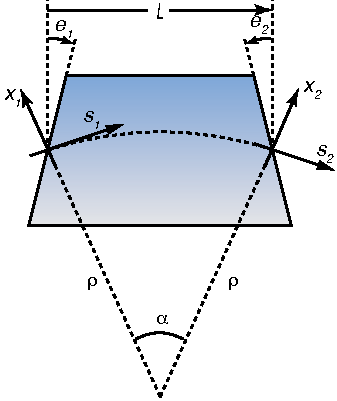
\includegraphics{rbend-coords.pdf}}
  \hspace{1cm}
  \subfigure[sbend]
  {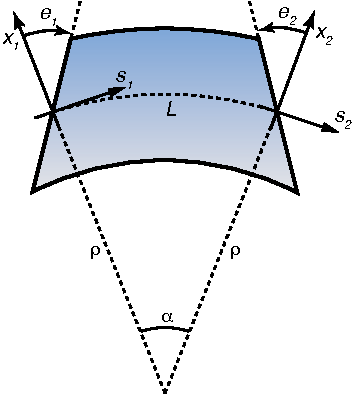
\includegraphics{sbend-coords.pdf}}
  \caption{Coordinate systems for (a) \vn{rbend} and (b) \vn{sbend} elements.}
  \label{f:bend}
\end{figure}

  \begin{description}
  \index{l}\index{l_chord}
  \item[l, l_chord]  \Newline
For an \vn{rbend}, \vn{l} is the chord length and not the arc length as
it is for an \vn{sbend}.  However, after reading in a lattice, \bmad will
internally convert all \vn{rbend}s into \vn{sbend}s, additionally, the
\vn{l_chord} attribute will be set to the input \vn{l}, and \vn{l} 
will be set to the true path length (see above).
  \index{h1}\index{h2}
  \item[h1, h2] \Newline
The attributes \vn{h1} and \vn{h2} are the curvature of the entrance
and exit pole faces. They are present for compatibility with MAD but
are not yet implemented in terms of tracking and other calculations.
  \index{e1}\index{e2}
  \item[e1, e2] \Newline
The rotation angle of the entrance pole face is \vn{e1} and at the
exit face it is \vn{e2}. Zero \vn{e1} and \vn{e2} for an \vn{rbend}
gives a rectangular magnet  (Figure~\ref{f:bend}a). Zero \vn{e1} and \vn{e2}
for an \vn{sbend} gives a wedge shaped magnet (Figure~\ref{f:bend}b).
An \vn{sbend} with an \vn{e1} = \vn{e2} = \vn{angle}/2 is equivalent 
to an \vn{rbend} with \vn{e1} = \vn{e2} = 0 (see above).
This formula holds for both positive and negative angles.
  \index{angle}
  \item[angle] \Newline
The total design bend angle. A positive \vn{angle} represents a
bend towards negative $x$ values (see Figure~\ref{f:local.coords}).
  \index{k1}\index{b1_gradient}
  \item[k1, b1_gradient] \Newline
The normalized and unnormalized quadrupole strength.
  \index{k2}\index{b2_gradient}
  \item[k2, b2_gradient] \Newline
The normalized and unnormalized sextupole strength. 
  \index{g}\index{rho}\index{g_err}
  \item[g, g_err, rho] \Newline
The design bending radius which determines the reference coordinate
system is \vn{rho} (see \sref{s:ref}). \vn{g} = 1/\vn{rho} is
the curvature function and is proportional to the design dipole
magnetic field. The true field strength is given by
\vn{g}~+~\vn{g_err} so changing \vn{g_err} leaves the design orbit
unchanged but varies a particle's orbit.
  \index{fint}\index{fintx}\index{hgapx}\index{hgapx}
  \item[fint, fintx, \Newline hgap, hgapx] \Newline
The field integrals for the entrance and
exit pole faces are give by \vn{fint} and \vn{fintx} respectively
\Begineq
  F_{int} = \int_{pole} \! \! ds \, \frac{B_y(s) (B_{y0} - B_y(s))}
  {2 H_{gap} B_{y0}^2}
\Endeq
with a similar equation for \vn{fintx}. In the equation $B_{y0}$ is
the field in the interior of the dipole and $H_{gap}$ is the pole half
gap.  The parameters \vn{hgap} and \vn{hgapx} are the half gaps at the
entrance and exit faces. If \vn{fint} or \vn{fintx} is given without a
value then a value of 0.5 is used. If \vn{fint} or \vn{fintx} is not
present, the default value of 0 is used. Note: \mad does not have the
\vn{fintx} and \vn{hgapx} attributes. \mad just assumes that the
values are the same for the entrance and exit faces. For compatibility
with \mad, if \vn{fint} is given but \vn{fintx} is not, then
\vn{fintx} is set equal to \vn{fint}. Similarly, \vn{hgapx} will be
set to \vn{hgap} if \vn{hgapx} is not given.

\index{Enge function}
\vn{fint} and \vn{hgap} can be related to the Enge function which is sometimes
used to model the fringe field. The Enge function is of the form
\Begineq
  B_y(s) = \frac{B_{y0}}{1 + \exp[P(s)]}
\Endeq
where
\Begineq
  P(s) = C_0 + C_1 \, s + C_2 \, s^2 + C_3 \, s^3 + \, \ldots
\Endeq
The C_0 term simply shifts where the edge of the bend is. If all the $C_n$
are zero except for $C_1$ then 
\Begineq
  C_1 = \frac{H_{gap}}{F_{int}}
\Endeq
  \index{tilt}
  \item[tilt] \Newline
The roll angle about the longitudinal axis at the entrance face of the
bend is given by \vn{tilt}.  \vn{tilt} = 0 bends the reference
trajectory in the $-x$ direction.  If the \vn{tilt} attribute is given
without any value then the value $\pi/2$ will be used. This makes for
a \vn{downward} pointing vertical bend. See Fig.~\ref{f:tilt.bend}.
  \end{description}

The attributes \vn{g}, \vn{angle}, and \vn{l} are mutually dependent. If any two are
specified for an element \bmad will calculate the appropriate value
for the third.  After reading in a lattice, \vn{angle} is considered a
dependent variable (\sref{s:depend}).

Since internally all \vn{rbend}s are converted to \vn{sbend}s, if one wants to
vary the \vn{g} attribute of a bend and still keep the bend rectangular, an
overlay (\sref{s:overlay}) can be constructed to maintain the proper face angles.
For example:
\begin{example}
  l_ch = 0.54
  g_in = 1.52
  l_coef = asin(l_ch * g_in / 2) / g_in
  my_bend: rbend, l = l_ch, g = g_in
  my_overlay: overlay = \{my_bend, my_bend[e1]:l_coef, my_bend[e2]:l_coef\}, g = g_in
\end{example}
Notice that \vn{l_coef} is just \vn{arc_length/2}.

\vn{n_ref_pass}, and \vn{ref_orbit} attributes are only used
when a bend is part of a \vn{multipass} line and is used to set the
reference geometry of the bend. See section~\sref{s:multipass} for
more details.

In the local coordinate system (\sref{s:ref}), looking from ``above''
(bend viewed from positive $y$), and with \vn{tilt} = 0, a positive
\vn{angle} represents a particle rotating clockwise. In this
case. \vn{g} will also be positive. For counterclockwise rotation,
both \vn{angle} and \vn{g} will be negative but the length \vn{l} is
always positive. Also, looking from above, a positive \vn{e1}
represents a clockwise rotation of the entrance face and a positive
\vn{e2} represents a counterclockwise rotation of the exit face. This
is true irregardless of the sign of \vn{angle} and \vn{g}. Also it is
always the case that the pole faces will be parallel when
\begin{example}
  e1 + e2 = angle
\end{example}

Example bend specification:
\begin{example}
  b03w: sbend, l = 0.6, k1 = 0.003, fint  ! gives fint = fintx = 0.5
\end{example}

%-----------------------------------------------------------------
\section{Branch and Photon_Branch}
\label{s:branch}
\index{branch|hyperbf}
\index{photon_branch|hyperbf}

A \vn{branch} element marks the start of an alternative line for the
particle beam.  A \vn{photon_branch} element marks the start of a
photon beam line. See \sref{s:branching} for more details.

General \vn{branch} and \vn{photon_branch} attributes are:
\begin{center}
\tt
\begin{tabular}{|l|l||l|l|} \hline
  {\sl Attribute Class}  & \s              & {\sl Attribute Class}      & \s              \HH
  Description strings    & \ref{s:string}  & Offsets                    & \ref{s:offset}  \HH
  Reference energy       & \ref{s:energy}  & Tracking \& transfer map   & \ref{c:methods} \HH
  Aperture Limits        & \ref{s:limit}   & Length                     & \ref{s:l}       \HH
                         &                 & Is_on                      & \ref{s:is.on}   \HH 
\end{tabular}
\end{center}
\toffset

%-----------------------------------------------------------------
\section{Capillary}
\label{s:capillary}
\index{capillary|hyperbf}

A \vn{capillary} element is a glass tube that is used to focus x-ray
beams.

General \vn{capillary} attributes are:
\begin{center}
\tt
\begin{tabular}{|l|l||l|l|} \hline
  {\sl Attribute Class}  & \s              & {\sl Attribute Class}      & \s              \HH
  Description strings    & \ref{s:string}  & Offsets                    & \ref{s:offset}  \HH
  Reference energy       & \ref{s:energy}  & Tracking \& transfer map   & \ref{c:methods} \HH
  Aperture Limits        & \ref{s:limit}   & Is_on                      & \ref{s:is.on}   \HH 
\end{tabular}
\end{center}
\toffset

\index{critical_angle_factor|hyperbf}
Attributes specific to a \vn{capillary} element are:
\begin{example}
  critical_angle_factor = <Real>    ! Critical angle * Energy (rad * eV)
\end{example}
The critical angle above which photons striking the capillary surface are
refracted into the capillary material scales as 1/Energy. The
constant of critical angle * energy is given by the \vn{critical_angle_factor}.

The inside wall of a capillary is defined by a number of
cross-sectional slices as shown in Fig.~\ref{f:capillary}A. Each
cross-section is defined by a number of vertices. The arc between each
vertex may be either a straight line, an arc of a circle, or a section
of an ellipse. It is mandatory that a cross-section be convex. That
is, given any two points within the cross-section, all points on the
line segment connecting them must be within the cross-section.

\index{wall}\vn{section}\index{s (capillary attribute)}\index{v (capillary attribute)}
\index{s_spline}\index{n_slice_spline}
The capillary \vn{wall structure} defines the capillary wall.  The
syntax of the wall structure is:
\begin{example}
  wall = \{
    section = \{ 
      s = <longitudinal_position>, 
      v(1) = \{<x>, <y>, <radius_x>, <radius_y>, <tilt>\}, 
      v(2) = \{ ... \},
      ...\},
    s_spline = \{<coef_1>, <coef_2>\},
    n_slice_spline = <num>,
    section = \{
      s = <longitudinal_position>, 
      v(1) = \{... \},
      ... \},
    ... \}
\end{example}
Note: Specifying \vn{s_spline} and \vn{n_cut_spline} is optional.
Example:
\begin{example}
  this_cap: capillary, 
    wall = \{   
      section = \{ ! cross-section with top/bottom symmetry
        s = 0, v(1) =  \{0.02, 0.00\}, 
        v(2) = \{0.00, 0.02, 0.02\}, v(3) = \{-0.01, 0.01\} \}, 
      s_spline = \{0.1, 0.7\}, 
      n_slice_spline = 4,
      section = \{  ! Cross-section that is a tilted ellipse.
        s = 0.34, 
        v(1) = \{0.003, -0.001, 0.015, 0.008, 0.2*pi\} \} \}
\end{example}

\begin{figure}[tb]
  \centering
  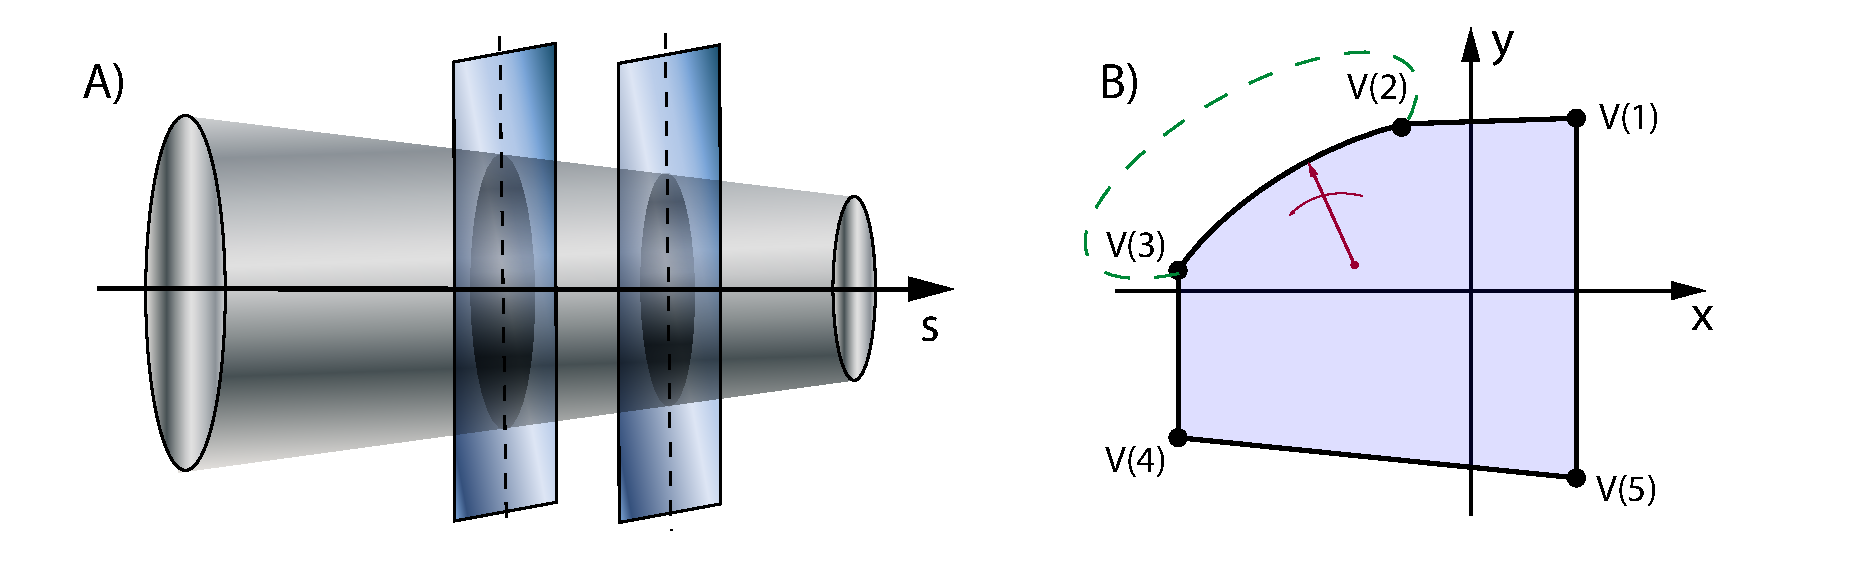
\includegraphics[width=6in]{capillary.pdf}
  \caption[cross-sectional slices of a capillary.]
{A) The inside wall of a capillary is defined by a number of
cross-sectional slices.  B) Each cross-section is made up of a number
of vertices. The segments between the vertices can be either a line
segment, the arc of a circle, or a section of an ellipse. The red line
segment with one end at the center of the arc and the other end
traversing the arc from, in this case $V(2)$ to $V(3)$, rotates in
counter clockwise manner. There are two solutions for constructing an
arc between two vertices. The solution with the center point furthest
from the origin, the dashed line between $V(2)$ and $V(3)$ in the
figure, is rejected.}
  \label{f:capillary}
\end{figure}

The capillary wall structure begins with ``\vn{wall = \{}'' and ends
with a ``\vn{\}}''. In between are a number of individual cross-section
structures.  Each individual cross-section begins with ``\vn{section =
\{}'' and ends with a ``\vn{\}}''. The \vn{s} parameter of a
cross-section gives the longitudinal position of the cross-section.
\vn{s} must be zero for the first cross-section and the length of the
capillary is given by the value of \vn{s} of the last cross-section.

The \vn{v(<j>)} within a cross-section define the vertices
for each cross-section. Each \vn{v(<j>)} in turn has five
parameters. It is mandatory to specify the first two parameters
\vn{<x>} and \vn{<y>}. Specifying the rest, \vn{<radius_x>},
\vn{<radius_y>}, and \vn{<tilt>}, is optional. The default values, if
not specified, is zero. The point (\vn{<x>}, \vn{<y>}) defines the
position of the vertex. The parameters \vn{<radius_x>},
\vn{<radius_y>}, and \vn{<tilt>} define the shape of the segment of
the cross-section between the given vertex and the preceding one.
\begin{example}
  <radius_x>  = 0, <radius_y>  = 0   --> Straight line segment.
  <radius_x> != 0, <radius_y>  = 0   --> Circular arc with radius = radius_x
  <radius_x>  = 0, <radius_y> != 0   --> Illegal!
  <radius_x> != 0, <radius_y> != 0   --> Ellipse section.
\end{example}
When an ellipse is specified, \vn{<radius_x>}, and \vn{<radius_y>} are
the half width and half height of the semi-major axes and the
\vn{<tilt>} parameter gives the tilt of the ellipse. \vn{<radius_x>}
and \vn{<radius_y>} must not be negative.

In the example above, for the first cross-section, \vn{v(2)}
specifies a non-zero \vn{<radius_x>} and, by default, \vn{<radius_y>}
is zero. Thus the segment of the cross-section between \vn{v(1)} and
\vn{v(2)} is circular in nature with a radius of 0.02. Since \vn{v(3)}
does not specify \vn{<radius_x>} nor \vn{<radius_y>}, the
cross-section between \vn{v(2)} and \vn{v(3)} is a straight line
segment.

The vertex points must be arranged in a ``counter clockwise manner''. 
For vertices \vn{<v(i)>} and \vn{<v(i+1)>} connected by a line segment
this translates to
\Begineq
  0 < \theta_{i+1} - \theta_{i} \pmod{2\pi} < \pi
\Endeq
where $(r_n, \theta_n)$ are the polar coordinates of the $n^{th}$
vertex. For vertices connected by an arc, ``counter clockwise manner''
means that the line segment with one end at the center of the arc and
the other end traversing the arc from \vn{<v(i)>} to \vn{<v(i+1)>}
rotates in counter clockwise as shown in Fig.~\ref{f:capillary}B. In
general, there are two solutions for constructing such an arc. The
solution chosen is the one whose center is closest to the origin.
With these restrictions, and with the restriction that the cross-section be convex,
it can be shown that the origin $(0,0)$ will be in the interior of any
cross-section and that for any cross-section a line drawn from the origin at
any given angle $\theta$ will intersect the cross-section at exactly
one point as shown in Fig.~\ref{f:capillary}B. This is an important
point in the construction of the capillary wall between cross-sections
as explained below.

The last vertex specified, call it \vn{<v(n)>}, should not have the
same \vn{<x>}, \vn{<y>} values as the first vertex \vn{<v(1)>}. That
is, there will be a segment of the cross-section connecting
\vn{<v(n)>} to \vn{<v(1)>}. The geometry of this segment is determined
by the parameters of \vn{<v(1)>}.

If there is mirror symmetry about the $x$ or $y$ axis for a
cross-section, the ``mirrored'' vertices, on the ``negative'' side of
the mirror plane, do not have to be specified. Thus if all the vertex
points of a cross-section are in the first quadrant, that is, all
\vn{<x>} and \vn{<y>} are zero or positive, mirror symmetry about both the
$x$ and $y$ axes is assumed. If all the \vn{<y>} values are zero or
positive and some \vn{<x>} values are positive and some are negative,
mirror symmetry about the $x$ axis is assumed. Finally, if all the
\vn{<x>} values are zero or positive but some \vn{<y>} values are
positive and some are negative, symmetry about the $y$ axis is
assumed. For example, for the first in the above example, since
all the \vn{<y>} values are non-negative and there are positive and
negative \vn{<x>} values, symmetry about the $x$ axis is assumed.

The one exception to the above rule that (\vn{<x>}, \vn{<y>}) is the
vertex center is when a single vertex \vn{v(1)} is specified for a
cross-section with a non-zero \vn{<radius_x>}. In this case,
(\vn{<x>}, \vn{<y>}) are taken to be the center of the circle or
ellipse. In the example above, the second cross-section is a
tilted ellipse with center at $(0.003, -0.001)$. If a cross-section
has a single vertex and \vn{<radius_x>} is
not specified, the cross-section is a rectangle. For example
\begin{example}
    section = \{ s = 0.34, v(1) = \{0.03, 0.01\} \}
\end{example}

\begin{figure}[tb]
  \centering
  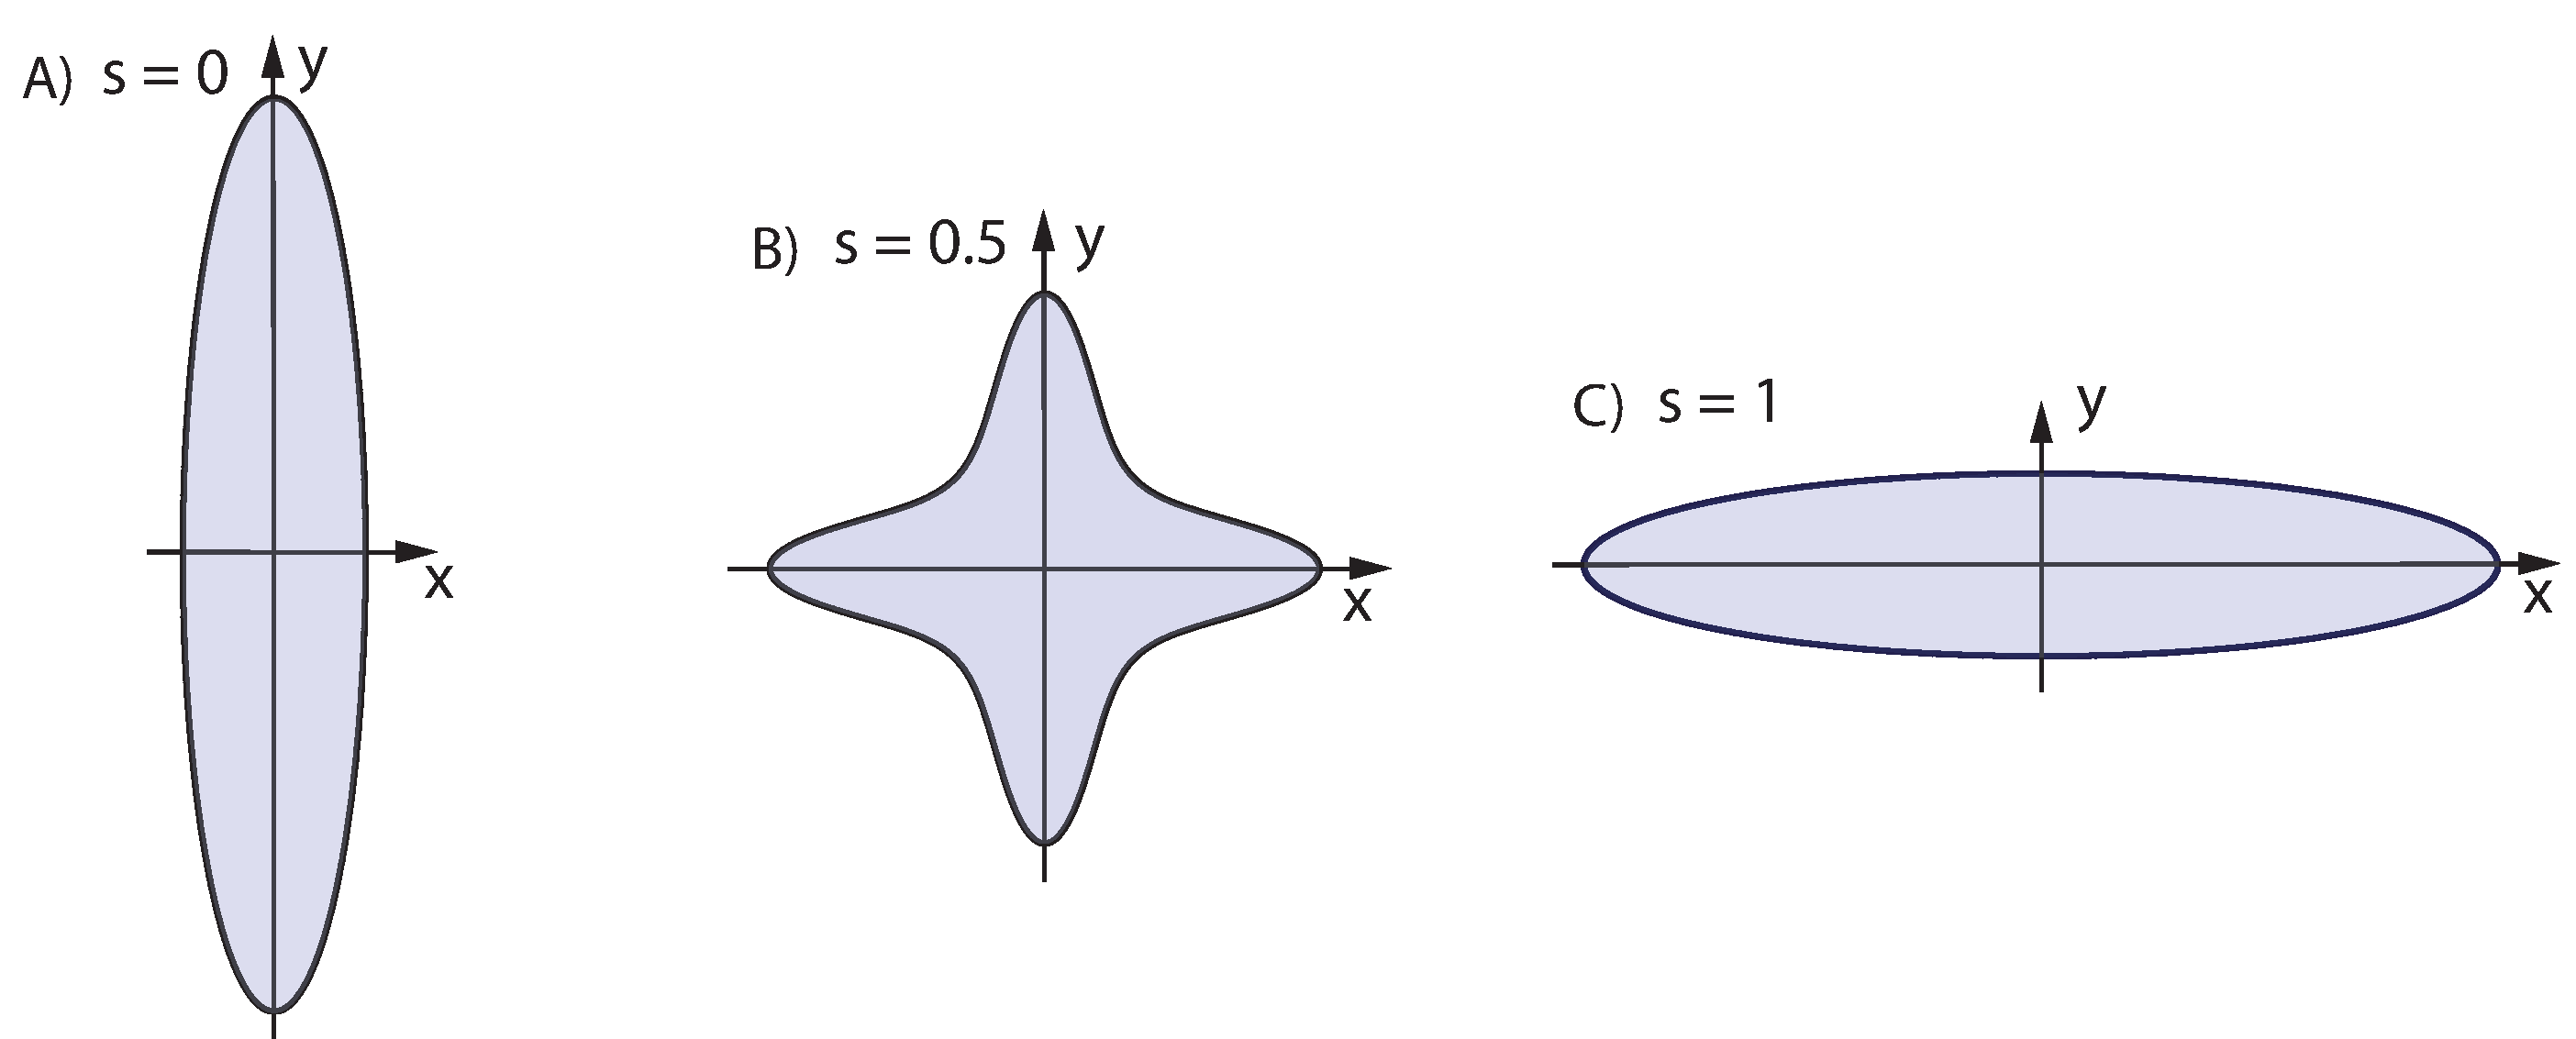
\includegraphics[width=4in]{concave-capillary.pdf}
  \caption[Convex cross-sections do not guarantee a convex volume.]
{Example where convex cross-sections do not produce a convex volume.
Cross-sections (A) and (C) are ellipses with a 5 to 1 aspect ratio.
Half way in between, linear interpolation produces a convex cross-section
as shown in (B).} 
  \label{f:concave-capillary}
\end{figure}

Between cross-sections, the capillary wall is defined by
interpolation. The default is a linear interpolation scheme.  let
$r_{c1}(\theta)$ be the radius of the capillary as a function of
$\theta$ for a given cross-section defined at $s = s_1$. Let
$r_{c2}(\theta)$ be the radius function at the next defined
cross-section at $s = s_2$. The capillary wall $r_c(\theta, s)$ at any
point $s$ between $s_1$ and $s_2$ is defined by the equation
\Begineq
  r_c(\theta, s) \equiv (1 - \stilde) \, r_{c1}(\theta) + \stilde \, r_{c2}(\theta)
\Endeq
where
\Begineq
  \stilde \equiv \frac{s - s_1}{s_2 - s_1}
\Endeq
In order for \bmad to quickly track photons through the capillary,
\bmad assumes that the volume between the cross-sections is
convex. The volume will be convex if each cross-section $r_c(\theta,
s)$ at any given $s$ is convex. Note that it is {\em not} sufficient
for $r_c(\theta, s)$ to be convex at the specified cross-sections as
shown in Fig.~\ref{f:concave-capillary}. Also note that it is perfectly
fine for the total capillary volume to not be convex.

To help reduce the complexity of specifying a capillary, ``virtual''
cross-sections may be defined by specifying a cubic interpolating
spline between two consecutive cross-sections and by specifying a
value for \vn{n_slice_spline}. The region between the two
cross-sections will then be divided into \vn{n_slice_spline} equal
longitudinal length regions. Between each region virtual
cross-sections are constructed defined by
\Begineq
  r_c(\theta, s) = (1 - P(\stilde)) \, r_{c1}(\theta) + P(\stilde) \, r_{c2}(\theta)
  \label{r1prp}
\Endeq
where $s$ is the longitudinal position of the phantom cross-section and
$P(s)$ is a cubic polynomial spline
\Begineq
  P(\stilde) = c_1 \, \stilde + c_2 \, \stilde^2 + c_3 \, \stilde^3
\Endeq
where $c_1$, $c_2$, and $c_3$ are constants. The $c_0$ constant has
been set to zero by the requirement that $P(0) = 0$. The requirement
that $P(1) = 1$ constrains $c_3$:
\Begineq
  c_3 = 1 - (c_1 + c_2)
\Endeq
 $c_1$ and $c_2$ are given by the \vn{s_spline} parameter between 
cross-sections. If not defined, the default is linear interpolation
with $c_1 = 1$ and $c_2 = 0$. Linear interpolation, is used to define
the wall between virtual cross-sections just as it is used for regular
cross-sections.

A non-linear interpolation scheme is used if \vn{n_splice_spline} is
set to 0.  In this case, the wall between the cross-sections is
constructed using \Eq{r1prp}. The volume between the cross-sections so
constructed must be convex.

To refer to a cross-section parameters after an element has been
defined, the following syntax is used:
\begin{example}
  ele_name[wall.section(n).v(j).x]   ! x value of j^th vertex of n^th cross-section
  ele_name[wall.n_slice_spline(n)]   ! n_slice_spline value set between n^th and 
                                     !     n+1^th cross-sections.
  ele_name[wall.s_spline(n).coef(k)] ! k^th coefficient (k = 1, 2, or 3) of s_spline 
                                     !     set between n^th and n+1^th cross-sections.
\end{example}

%-----------------------------------------------------------------
\section{Collimators: Ecollimator and Rcollimator} \label{s:col}
\index{ecollimator|hyperbf}
\index{rcollimator|hyperbf}

An \vn{ecollimator} is a drift with elliptic collimation. An
\vn{rcollimator} is a drift with rectangular collimation.

General \vn{ecollimator} and \vn{rcollimator} attributes are:
\begin{center}
\tt
\begin{tabular}{|l|l||l|l|} \hline
  {\sl Attribute Class}  & \s              & {\sl Attribute Class}      & \s              \HH
  Description strings    & \ref{s:string}  & Offsets                    & \ref{s:offset}  \HH
  Reference energy       & \ref{s:energy}  & Tracking \& transfer map   & \ref{c:methods} \HH
  Aperture Limits        & \ref{s:limit}   & Length                     & \ref{s:l}       \HH
  Symplectify            & \ref{s:symp}    & Integration settings       & \ref{s:integ}   \HH
  Hkick \& Vkick         & \ref{s:kick}    &                            &                 \HH
\end{tabular}
\end{center}
\toffset

Note: Collimators are the exception to the rule that the aperture is
independent of any \vn{tilt}s. See \sref{s:limit} for more
details. Example:
\begin{example}
  d21: ecollimator, l = 4.5, x_limit = 0.09/2, y_limit = 0.05/2
\end{example}

%-----------------------------------------------------------------
\section{Crystal}
\label{s:crystal}
\index{crystal|hyperbf}

\begin{figure}[tb]
  \centering
  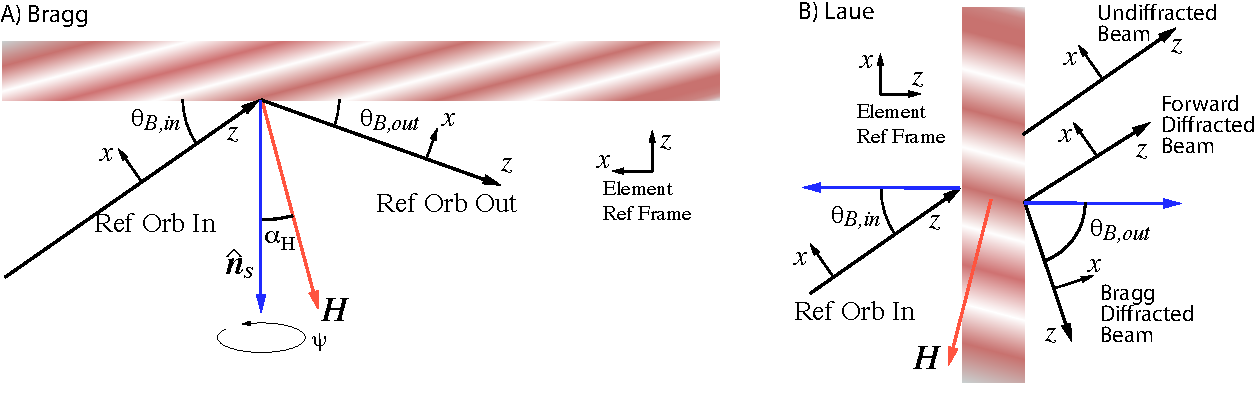
\includegraphics[width=5in]{crystal-ele.pdf}
  \caption[Crystal element geometry.]
{Crystal element geometry for Bragg reflections. 
The geometry shown is appropriate for zero
\vn{tilt} (reference trajectory in the $x$-$z$ plane). The angle
$\alpha_H$ (\vn{alpha_angle}) is the angle of the $\bfH$ vector with
respect to the surface normal $\bfhat n$. For $\psi$ (\vn{psi_angle})
zero, the incoming reference orbit, the outgoing reference orbit,
$\bfhat n$, and $\bfH$ are all coplanar. The element reference coordinates
where $\bfhat x$ is parallel to the surface normal establishes the coordinates
for specifying a rotation of $\bfH$ around the surface normal and specifying
a curvature of the surface.}
  \label{f:crystal}
\end{figure}

A \vn{crystal} element represents a crystal used for photon diffraction.

General \vn{crystal} attributes are:
\begin{center}
\tt
\begin{tabular}{|l|l||l|l|} \hline
  {\sl Attribute Class}  & \s              & {\sl Attribute Class}      & \s              \HH
  Description strings    & \ref{s:string}  & Offsets                    & \ref{s:offset}  \HH
  Reference energy       & \ref{s:energy}  & Tracking \& transfer map   & \ref{c:methods} \HH
  Aperture Limits        & \ref{s:limit}   & Symplectify                & \ref{s:symp}    \HH
\end{tabular}
\end{center}
\toffset

\index{graze_angle_err}\index{psi_angle}
\index{b_param}\index{bragg_angle}\index{crystal_type}
\index{tilt_err}\index{g_graze}\index{g_trans}
\index{d_detec}\index{d_source}
\index{c2_curve}\index{c3_curve}\index{c4_curve}
\index{follow_diffracted_beam}\index{thickness}
Attributes specific to a \vn{crystal} element are:
\begin{example}
  b_param                = <Real>    ! b parameter
  crystal_type           = <String>  ! Crystal material and reflection plane.
  c2_curve               = <Real>    ! C2 curvature coefficient.
  c3_curve               = <Real>    ! C3 curvature coefficient.
  c4_curve               = <Real>    ! C4 curvature coefficient.
  d_detec                = <Real>    ! Detector distance.
  d_source               = <Real>    ! Source distance.
  g_trans                = <Real>    ! 1/Radius-of-curvature transverse to the bend plane.
  graze_angle_err        = <Real>    ! Error in the graze angle.
  psi_angle              = <Real>    ! Rotation of H-vector about the surface normal.
  tilt_err               = <Real>    ! Error in the tilt angle.
  thickness              = <Real>    ! Thickness of crystal for Laue diffraction.
  follow_diffracted_beam = <Logic>   ! Track the diffracted or undiffracted beam?
  negative_graze_angle  = <Logic>    ! Use negative graze angle? Default is False.
\end{example}

\index{graze_angle_in}\index{graze_angle_out}\index{alpha_angle}
\index{tilt_corr}\index{d_spacing}\index{v_unitcell}\index{f0_re}
\index{f0_im}\index{fh_re}\index{fh_im}\index{ref_wave_length}
\index{c2_curve_tot}\index{c3_curve_tot}\index{c4_curve_tot}
Dependent variables (\sref{s:depend}) specific to a \vn{crystal} element are:
\begin{example}
  alpha_angle      ! Angle of H-vector with respect to the surface normal.
  bragg_angle      ! Nominal Bragg angle at the reference wave length. 
  c2_curve_tot     ! Total C2 curvature coefficient.
  c3_curve_tot     ! Total C3 curvature coefficient.
  c4_curve_tot     ! Total C4 curvature coefficient.
  d_spacing        ! Lattice plane spacing. 
  f0_re            ! Real part of f0
  f0_im            ! Imaginary part of f0
  fh_re            ! Real part of fh
  fh_im            ! Imaginary part of fh
  graze_angle_in   ! Angle between incoming beam and mirror surface.
  graze_angle_out  ! Angle between incoming beam and mirror surface.
  ref_wavelength   ! Reference wavelength
  ref_cap_gamma    ! \(\Gamma\) at the reference wavelength.
  tilt_corr        ! Tilt correction due to a finite psi_angle.
  v_unitcell       ! Unit cell volume. 
\end{example}

The \vn{crystal_type} attribute defines the crystal material and
diffraction lattice plane. The syntax is \vn{"ZZijk"} where \vn{ZZ} is
the atomic symbol for the material and \vn{ijk} are the Miller indices
for the diffraction plane. For example, \vn{"si111"}. From this, and
the reference photon energy (\sref{s:energy}), the spacing between
lattice planes (\vn{d_spacing}), the unit cell volume
(\vn{v_unitcell}), and the structure factor\cite{b:batterman} values
\vn{f0_re}, \vn{f0_im}, \vn{fh_re}, \vn{fh_im} can be computed.

The \vn{b_param} is the standard asymmetry factor
\Begineq
  b = \frac{\sin(\alpha_H + \theta_B)}{\sin(\alpha_H - \theta_B)} 
\Endeq
where $\theta_B$ is the Bragg angle (\vn{bragg_angle}) 
\Begineq
  \theta_B = \frac{\lambda}{d \, \sin\theta}
\Endeq
and $\alpha_H$ (\vn{alpha_angle}) is the angle of the reciprocal
lattice $\bfH$ vector with respect to the surface normal as shown in
Fig.~\ref{f:crystal}.  If \vn{b_param} is set to -1 then there is
Bragg reflection and \vn{alpha_H} is zero. If \vn{b_param} is set to 1
then there is Laue diffraction again with \vn{alpha_H} zero. With the
orientation shown in Fig.~\ref{f:crystal}, \vn{alpha_H} is positive.

The \vn{thickness} parameter is used with Laue diffraction only.

The \vn{follow_diffracted_beam} parameter sets whether the diffracted
beam or the undiffracted beam tracked. This parameter is only relavent
with Laue diffraction.

If \vn{psi_angle} is zero, the incoming reference orbit, the outgoing
reference orbit, $\bfhat n$ and $\bfH$ are all coplanar. A non-zero
\vn{psi_angle} Rotates the $\bfH$ vector around the $+\bfhat x$ axis
of the \vn{Element Reference Frame} (See Fig.~\ref{f:crystal}).

The reference trajectory for a \vn{crystal} is that of a zero length
bend (\sref{s:mirror.coords}) and hence the length (\vn{l}) parameter
of a crystal is fixed at zero. The orientation of the reference
trajectory with respect to the crystal surface is specified by the
incoming graze angle \vn{graze_angle_in} ($\theta_{g,in}$) and
outgoing graze angle \vn{graze_angle_out} ($\theta_{g,out}$) as shown
in Fig.~\ref{f:crystal}. These angles are computed from the photon
reference energy and the other crystal parameters such that a photon
with the reference energy traveling along the reference trajectory
will be in the center of the Darwin curve (\sref{s:crystal.tracking}).
If \vn{negative_graze_angle} is set to \vn{True}, 
\vn{graze_angle_in} and \vn{graze_angle_out} will be negative. This is
equivalent to setting \vn{tilt} to \vn{pi}.

The reference trajectory in the global coordinate system
(\sref{s:global}) is determined by the value of the \vn{tilt}
parameter along with the value of \vn{graze_angle_in} +
\vn{graze_angle_out}. A positive \vn{graze_angle_in} +
\vn{graze_angle_out} bends the reference trajectory in the same
direction as a positive \vn{g} for a bend element. The
\vn{graze_angle_err} and \vn{tilt_err} parameters affect the
orientation of the \vn{crystal} in the global reference system but do
not affect the reference trajectory.

A \vn{crystal} may be offset and pitched (\ref{s:offset}). The incoming
local reference coordinates are used for these misalignments. The
\vn{x_pitch} and \vn{y_pitch} parameters can be related to the
\vn{graze_angle_err} and \vn{tilt_err} parameters. For example, with
zero \vn{tilt}, a positive \vn{x_pitch} is equivalent to a negative
\vn{graze_angle_err} of the same magnitude, and a positive
\vn{y_pitch} is equivalent to a negative \vn{tilt_err} of the same
magnitude.

The curvature of the surface in the plane of the $x$-$z$ plane of the
Element Reference Frame (see Fig.~\ref{f:crystal}) is determined by
the \vn{d_source}, \vn{d_detec}, \vn{c2_curve}, \vn{c2_curve}, and
\vn{c2_curve} parameters. The curvature is surface is parameterized by
a fourth order polynomial
\Begineq
  -x = c_{2,tot} \, z^2 + c_{3,tot} \, z^3 + c_{4,tot} \, z^4
\Endeq
The coefficients of the polynomial are determined by
\begin{align}
  c_{2,tot} &= \mbox{c2_curve} + \frac{1}{2 \, R_c} \CRNO
  c_{3,tot} &= \mbox{c3_curve} \\
  c_{4,tot} &= \mbox{c4_curve} + \frac{1}{4 \, R_c^3} \CRNO
\end{align}
where 
\Begineq
  \frac{2}{R_c} = \frac{\theta_{g,in}}{d_s} + 
                  \frac{\theta_{g,out}}{d_d}
\Endeq
and
\begin{align}
  d_s &= \begin{cases} 
    \infty & \mbox{d_source} = 0 \\
    \mbox{d_source} & \mbox{otherwise}
  \end{cases} \CRNO
  d_d &= \begin{cases} 
    \infty & \mbox{d_detec} = 0 \\
    \mbox{d_detec} & \mbox{otherwise}
  \end{cases}
\end{align}
\vn{d_source} and \vn{d_detec} can be thought of as distances from the
crystal to the photon source and detector of photons.  With the above
definitions, and with \vn{c2_curve}, \vn{c3_curve}, and \vn{c4_curve}
equal to zero, photons from the source will be focused on the
detector.

When a crystal is bent, The $\bfH$ vector is assumed follow the
curface curvature. That is, it is assumed that the lattice planes are
curved by the bending.

The \vn{g_graze} parameter is equal to 1/\vn{R_graze} where
\vn{R_graze} is the radius of curvature of the crystal surface in the
bend plane as shown in Fig.~\ref{f:mirror}. A positive \vn{g_graze}
indicates that the crystal is concave from the point of view of the
photons. Similarly, the \vn{g_trans} parameter is equal to
1/\vn{R_trans} where \vn{R_trans} is the radius of curvature of the
crystal surface in the plane transverse to the bend plane. Again, a
positive \vn{g_trans} indicates that the crystal is concave from the
point of view of the photons.

Example:
\begin{example}
  crystal_ele: crystal, crystal_type = 'si111', b_param = -1
\end{example}

%-----------------------------------------------------------------
\section{Custom}
\label{s:custom}
\index{custom|hyperbf}

A \vn{custom} element is an element whose properties are defined
outside of the standard \bmad subroutine library. That is, to use a
custom element, some programmer must write the appropriate custom
routines which are then linked with the \bmad subroutines into a
program. \bmad will call the custom routines at the appropriate time
to do tracking, transfer matrix calculations, etc. See the programmer
who wrote the custom routines for more details! See
\sref{s:custom.ele} on how to write custom routines.

General \vn{custom} attributes are:
\begin{center}
\tt
\begin{tabular}{|l|l||l|l|} \hline
  {\sl Attribute Class}  & \s              & {\sl Attribute Class}      & \s              \HH
  Symplectify            & \ref{s:symp}    & Offsets, pitches, and tilt & \ref{s:offset}  \HH
  Description strings    & \ref{s:string}  & Is_on                     & \ref{s:is.on}   \HH 
  Reference energy       & \ref{s:energy}  & Tracking \& transfer map   & \ref{c:methods} \HH
  Aperture Limits        & \ref{s:limit}   & Length                     & \ref{s:l}       \HH
  Integration settings   & \ref{s:integ}   &                            &                 \HH
\end{tabular}
\end{center}
\toffset

\index{delta_e}
\index{val1,  ..., Val12}
Attributes specific to a \vn{custom} element are
\begin{example}
  val1, ..., val12 = <Real>  ! Custom values 
  delta_e          = <Real>  ! Change in energy.
\end{example}

\vn{delta_e} is the energy gain of the {\it reference} particle
between the starting edge of the element and the ending edge.

Example:
\begin{example}
  c1: custom, l = 3, val4 = 5.6, val12 = 0.9, ds_step = 0.2, tracking_method = boris
\end{example}

%-----------------------------------------------------------------
\section{Drift}
\label{s:drift}
\index{drift|hyperbf}

A \vn{drift} element is a space free and clear of any fields.

General \vn{drift} attributes are:
\begin{center}
\tt
\begin{tabular}{|l|l||l|l|} \hline
  {\sl Attribute Class}  & \s              & {\sl Attribute Class}      & \s              \HH
  Reference energy       & \ref{s:energy}  & Tracking \& transfer map   & \ref{c:methods} \HH
  Aperture Limits        & \ref{s:limit}   & Length                     & \ref{s:l}       \HH
  Description strings    & \ref{s:string}  & Symplectify                & \ref{s:symp}    \HH 
  Integration settings   & \ref{s:integ}   & Hkick \& Vkick             & \ref{s:kick}    \HH
                         &                 & Offsets, pitches, and tilt & \ref{s:offset}  \HH
\end{tabular}
\end{center}
\toffset

Example:
\begin{example}
  d21: drift, l = 4.5
\end{example}

%-----------------------------------------------------------------
\section{Elseparator}
\label{s:elsep}
\index{elseparator|hyperbf}

An \vn{elseparator} is an electrostatic separator.

General \vn{elseparator} attributes are:
\begin{center}
\tt
\begin{tabular}{|l|l||l|l|} \hline
  {\sl Attribute Class}  & \s              & {\sl Attribute Class}      & \s              \HH
  Symplectify            & \ref{s:symp}    & Offsets, pitches, and tilt & \ref{s:offset}  \HH
  Description strings    & \ref{s:string}  & Is_on                     & \ref{s:is.on}   \HH 
  Reference energy       & \ref{s:energy}  & Tracking \& transfer map   & \ref{c:methods} \HH
  Aperture Limits        & \ref{s:limit}   & Length                     & \ref{s:l}       \HH
  Hkick \& Vkick         & \ref{s:kick}    & a$n$, b$n$ multipoles      & \ref{s:multip}  \HH
  Integration settings   & \ref{s:integ}   &                            &                 \HH
\end{tabular}
\end{center}
\toffset

\index{gap}
\index{e_field}
\index{voltage}
Attributes specific to an \vn{elseparator} element are:
\begin{example}
  gap = <Real> ! Distance between electrodes
  voltage      ! Voltage between electrodes. This is a dependent variable (\sref{s:depend}).
  e_field      ! Electric field. This is a dependent variable (\sref{s:depend}).
\end{example}

\index{hkick}
\index{vkick}
For an \vn{elseparator}, the kick is determined by \vn{hkick} and
\vn{vkick}. The \vn{gap} for an \vn{Elseparator} is used to compute
the electric field for a given kick. The voltage is a dependent
attribute determined by:
\begin{example}
  e_field (V/m) = sqrt(hkick^2 + vkick^2) * E_TOT / L
  voltage (V) = e_field * gap  
\end{example}

Example:
\begin{example}
  h_sep: elsep, l = 4.5, hkick = 0.003, gap = 0.11
\end{example}

%-----------------------------------------------------------------
\section{Hkicker and Vkicker}
\label{s:hvkicker}
\index{hkicker|hyperbf}
\index{vkicker|hyperbf}

An \vn{hkicker} gives a beam a horizontal kick and a \vn{vkicker} gives a 
beam a vertical kick.

General \vn{hkicker} \vn{vkicker} attributes are:
\begin{center}
\tt
\begin{tabular}{|l|l||l|l|} \hline
  {\sl Attribute Class}  & \s              & {\sl Attribute Class}      & \s              \HH
  Symplectify            & \ref{s:symp}    & tilt                       & \ref{s:offset}  \HH
  Description strings    & \ref{s:string}  & Is_on                     & \ref{s:is.on}   \HH 
  Reference energy       & \ref{s:energy}  & Tracking \& transfer map   & \ref{c:methods} \HH
  Aperture Limits        & \ref{s:limit}   & Length                     & \ref{s:l}       \HH
  Kick                   & \ref{s:kick}    & a$n$, b$n$ multipoles      & \ref{s:multip}  \HH
  Integration settings   & \ref{s:integ}   &                            &                 \HH
\end{tabular}
\end{center}
\toffset

\index{kick}
\index{hkick}
\index{vkick}
Note that \vn{hkicker} and \vn{vkicker} elements use the
\vn{kick} attribute while a \vn{kicker} uses the \vn{hkick} and \vn{vkick} 
attributes. Example:
\begin{example}
  h_kick: hkicker, l = 4.5, kick = 0.003
\end{example}

%-----------------------------------------------------------------
\section{Hybrid}
\label{s:hybrid}
\index{hybrid|hyperbf}

A \vn{hybrid} element is an element that is formed by concatenating
other element together. \vn{hybrid} elements are not part of the input
lattice file but are created by a program, usually for speed purposes.

%-----------------------------------------------------------------
\section{Girder}
\label{s:girder}
\index{girder|hyperbf}

A \vn{girder} is a support structure that orients the elements that
are attached to it in space.

General \vn{girder} attributes are:
\begin{center}
\tt
\begin{tabular}{|l|l||l|l|} \hline
  {\sl Attribute Class}  & \s              & {\sl Attribute Class}      & \s              \HH
  Description strings    & \ref{s:string}  & Offsets, pitches, and tilt & \ref{s:offset}  \HH 
\end{tabular}
\end{center}
\toffset

Attributes specific to a \vn{girder} are:
\begin{example}
  girder = \{<List>\}   ! List of elements on the Girder
\end{example}

\index{x_offset}
\index{y_pitch}
\index{tilt}
When a \vn{girder} overlays an element, then that elements
orientation attributes (\vn{x_offset}, \vn{y_pitch}, \vn{tilt}, etc.) 
give the orientation of
the element with respect to the \vn{girder}. An example will make this clear:
\begin{example}
  q1: quad, l = 10
  q2: quad, l = 5, x_offset = 0.2, x_pitch = 0.01
  ib: girder = \{q1, q2\}, x_pitch = 0.1, x_offset = 0.3
  this_line: line = (q1, q2)
  use, this_line
\end{example}
\index{overlay}
In this example \vn{ib} supports elements \vn{q1} and \vn{q2}. The
center of \vn{ib} is at $s = 7.5$ (\vn{ib} starts at $s = 0$ which is
the beginning of \vn{q1} and ends at $s = 15$ which is the end of
\vn{q2}). Like other elements, pitch is calculated from the center of
a \vn{girder} element (see Sec.~\ref{s:offset}). The center of
\vn{q2} is at $s = 12.5$ so the distance between the center of \vn{ib}
and \vn{q2} is $ds = 5$. The pitch of \vn{ib} produces an offset at
the center of \vn{q2} of $0.5 = 0.1 * 5$. This, added to the offsets
of \vn{ib} and \vn{q2}, give the total offset of \vn{q2} to be $1.0 =
0.5 + 0.3 + 0.2$. The total \vn{x_pitch} of \vn{q2} is $0.11 = 0.1 +
0.01$. From the above example it can be seen that a \vn{girder} looks
similar to an \vn{Overlay} (see Sec.~\ref{s:overlay}). It would,
however, take six \vn{Overlays} to simulate the effect of a single
\vn{girder}.

The \vn{girder} statement syntax is:
\begin{example}
  <element_name>: GIRDER = \{<ele1>, <ele2>, ... \}, ...
\end{example}
A \vn{girder} element will be created for each \vn{<ele1>} element in
the lattice. The elements \vn{<ele2>}, \vn{<ele3>}, etc. do not have to be
consecutive but, if more than one \vn{girder} is to be created, need
to be in order of increasing \vn{s}.
For example:
\begin{example}
  q1: quad
  q2: quad
  s0: sextupole
  s1: sextupole
  ib: girder = \{q1, s1, q2\}
  this_line: line = (q1, s0, s1, q2, ..., q1, s0, s1, q2)
  use, this_line
\end{example}
In this example two \vn{girder} elements will be created.

Note to programmers: The total horizontal offset of any element is
stored in the element component \vn{%value(x_offset_tot\$)}. Similarly
the total tilt is stored in \vn{%value(tilt_tot\$)}, etc.

%-----------------------------------------------------------------
\section{Instrument, Monitor, and Pipe}
\label{s:monitor}
\index{instrument|hyperbf}
\index{monitor|hyperbf}
\index{pipe|hyperbf}

\bmad treats \vn{instrument}, \vn{monitor}, and \vn{pipe} elements
like a \vn{drift}. There is a difference, however, when superimposing
elements (\sref{s:super}). For example, a \vn{quadrupole} superimposed
on top of a \vn{drift} results in a free \vn{quadrupole} element in
the tracking part of the lattice and no lord elements are created. On
the other hand, a \vn{quadrupole} superimposed on top of a
\vn{monitor} results in a \vn{quadrupole} element in the tracking part
of the lattice and this \vn{quadrupole} element will have two lords: A
\vn{quadrupole} superposition lord and a \vn{monitor} superposition
lord.

General \vn{instrument}, \vn{monitor}, and \vn{pipe} attributes are:
\begin{center}
\tt
\begin{tabular}{|l|l||l|l|} \hline
  {\sl Attribute Class}  & \s               & {\sl Attribute Class}      & \s              \HH
  Symplectify            & \ref{s:symp}     & Offsets, pitches, and tilt & \ref{s:offset}  \HH
  Reference energy       & \ref{s:energy}   & Tracking \& transfer map   & \ref{c:methods} \HH
  Aperture Limits        & \ref{s:limit}    & Length                     & \ref{s:l}       \HH
  Description strings    & \ref{s:string}   & Is_on                      & \ref{s:is.on}   \HH 
  Integration settings   & \ref{s:integ}    & Hkick \& Vkick             & \ref{s:kick}    \HH
  Instrumental variables & \ref{s:meas.attrib} &                         &                 \HH
\end{tabular}
\end{center}
\toffset

\index{x_offset}
\index{y_offset}
\index{x_pitch}
\index{y_pitch}
\index{tilt}
The \vn{offset}, \vn{pitch}, and \vn{tilt} attributes are not
used by any \bmad routines. If these attributes are used by a program
they are typically used to simulate such things as measurement
offsets. The \vn{is_on} attribute is also not used by \bmad
proper. Example:
\begin{example}
  d21: instrum, l = 4.5
\end{example}

%-----------------------------------------------------------------
\section{Kicker}
\label{s:kicker}
\index{kicker|hyperbf}

\index{hkick}
\index{vkick}
\index{h_displace}
\index{v_displace}
A \vn{kicker} can deflect a beam in both planes. Note that a
\vn{kicker} uses the \vn{hkick} and \vn{vkick} attributes while
\vn{hkicker} and \vn{vkicker} elements use the \vn{kick} attribute. 
In addition a \vn{kicker} can apply a displacement to a particle
using the \vn{h_displace} and \vn{v_displace} attributes.

General \vn{kicker} attributes are:
\begin{center}
\tt
\begin{tabular}{|l|l||l|l|} \hline
  {\sl Attribute Class}  & \s              & {\sl Attribute Class}      & \s              \HH
  Symplectify            & \ref{s:symp}    & tilt                       & \ref{s:offset}  \HH
  Description strings    & \ref{s:string}  & Is_on                     & \ref{s:is.on}   \HH 
  Reference energy       & \ref{s:energy}  & Tracking \& transfer map   & \ref{c:methods} \HH
  Aperture Limits        & \ref{s:limit}   & Length                     & \ref{s:l}       \HH
  Hkick \& Vkick         & \ref{s:kick}    & a$n$, b$n$ multipoles      & \ref{s:multip}  \HH
  Integration settings   & \ref{s:integ}   &                            &                 \HH
\end{tabular}
\end{center}
\toffset

Example:
\begin{example}
  a_kick: kicker, l = 4.5, hkick = 0.003
\end{example}

%-----------------------------------------------------------------
\section{Lcavity}
\label{s:lcav}
\index{lcavity|hyperbf}

An \vn{lcavity} is a LINAC accelerating cavity.
The main difference between an \vn{rfcavity} and an
\vn{lcavity} is that, unlike an \vn{rfcavity}, the reference energy
(\sref{s:phase.space}) through an \vn{lcavity} is not constant.

General \vn{lcavity} attributes are:
\begin{center}
\tt
\begin{tabular}{|l|l||l|l|} \hline
  {\sl Attribute Class}  & \s                 & {\sl Attribute Class}      & \s               \HH
  Symplectify            & \ref{s:symp}       & Offsets, and pitches       & \ref{s:offset}   \HH
  Description strings    & \ref{s:string}     & Is_on                      & \ref{s:is.on}    \HH 
  Reference energy       & \ref{s:energy}     & Tracking \& transfer map   & \ref{c:methods}  \HH
  Aperture Limits        & \ref{s:limit}      & Length                     & \ref{s:l}        \HH
  Hkick \& Vkick         & \ref{s:kick}       & Integration settings       & \ref{s:integ}    \HH
  RF Couplers            & \ref{s:rf.coupler} & RF Wakes                   & \ref{s:rf.wakes} \HH
  RF Fields              & \ref{s:rf.fields}  &                            &                  \HH
\end{tabular}
\end{center}
\toffset

The attributes specific to an \vn{lcavity} are 
\index{gradient}\index{phi0}
\index{dphi0}\index{e_loss}
\index{rf_frequency}\index{delta_e}
\begin{example}
  gradient         = <Real>   ! Accelerating gradient (V/m).
  gradient_err     = <Real>   ! Accelerating gradient error (V/m).
  phi0             = <Real>   ! Phase (rad/2\(\pi\)) of the reference particle with 
                              !   respect to the RF. phi0 = 0 is on crest.
  dphi0            = <Real>   ! Phase with respect to a multipass lord (rad/2\(\pi\)).
  phi0_err         = <Real>   ! Phase error (rad/2\(\pi\))
  e_loss           = <Real>   ! Loss parameter for short range wake fields (V/Coul).
  rf_frequency     = <Real>   ! Rf frequency (Hz).
  delta_e                     ! Change in energy of an on-crest particle. 
                              !   Dependent attribute (\sref{s:depend}).
\end{example}
The dependent variable \vn{delta_e} attribute can be used in place of
\vn{gradient} as discussed in \sref{s:depend}.  \vn{delta_e} is a
dependent attribute and is defined to be
\begin{example}
  delta_e = gradient * L
\end{example}

The energy kick felt by a particle is 
\begin{example}
  dE = gradient_tot * L * cos(twopi * (phi(z) + phi_ref + phi0_err) - 
                                                     e_loss * n_part * e_charge 
  \label{egl2p}
\end{example}
\index{multipass}
where
\begin{example}
  gradient_tot = gradient + gradient_err
  phi(z) = -z * rf_frequency / velocity
  phi_ref = phi0 + dphi0
\end{example}
Where z is the particles's $z$ phase space coordinate (\sref{s:phase.space}).
See \sref{s:rf.time} for a discussion on timing issues.
\vn{dphi0} is only to be used to shift the phase with respect to a
\vn{multipass} lord. See \sref{s:multipass}.

The \vn{e_loss} attribute in the formula for \vn{dE} represents the
energy loss due to short--range wake fields. \vn{n_part} is set using
the \vn{parameter} statement (\sref{s:param}) and represents the
number of particles in a bunch. \vn{e_charge} is the charge on an
electron (Table~\ref{t:constants}). Notice that the energy kick is
independent of the sign of the charge of the particle

The energy change of the reference particle is just the energy change for a 
particle with $z = 0$ and no phase or gradient errors. Thus
\begin{example}
  dE(reference) = gradient * L * cos(twopi * phi_ref) - e_loss * n_part * e_charge
\end{example}

The energy kick for a \bmad \vn{lcavity} is consistent with MAD. 
Note: The MAD8 documentation for an \vn{lcavity} has a wrong
sign. Essentially the MAD8 documentation gives
\begin{example}
  dE = gradient * L * cos(twopi * (phi_ref - phi(z))) ! WRONG
\end{example}
This is incorrect. 

The transverse trajectory through an \vn{lcavity} is modeled using
equations developed by Rosenzweig and Serafini\cite{b:rosenzweig}
modified to give the correct phase-space area at non
ultra-relativistic energies.  See Section \sref{s:lcav.phys} for more
details.  Note: The transfer matrix for an \vn{lcavity} with finite
\vn{gradient} is never symplectic. See \sref{s:phase.space}. In
addition, couplers (\sref{s:rf.coupler}) and HOM wakes
(\sref{s:rf.wakes}) can be modeled.

\index{RF field map}
\index{runge_kutta!and field maps}\index{adaptive_boris!and field maps}
\index{boris!and field maps}\index{symp_lie_bmad!and field maps}
\index{symp_lie_bmad}
If a field map is specified (\sref{s:rf.fields}), tracking using an
integrator is possible. A field map is only used for \vn{runge_kutta},
\vn{adaptive_boris}, \vn{boris} and \vn{symp_lie_bmad} tracking
(\sref{s:tkm}).  For \vn{symp_lie_bmad} tracking, only the
accelerating mode(s) are used.  This is done for a practical reason:
Only the fundamental mode has an analytical formula for the symplectic
tracking. In the future, the other modes could be used with
\vn{symp_lie_bmad} tracking using a field expansion about the
centerline.


%-----------------------------------------------------------------
\section{Marker}
\label{s:mark}
\index{marker|hyperbf}

A \vn{marker} is a zero length element meant to mark a position. 

General \vn{marker} attributes are:
\begin{center} 
\tt
\begin{tabular}{|l|l||l|l|} \hline
  {\sl Attribute Class}  & \s               & {\sl Attribute Class}      & \s              \HH
  Description strings    & \ref{s:string}   & Is_on                      & \ref{s:is.on}   \HH 
  Reference energy       & \ref{s:energy}   & Offsets and tilt           & \ref{s:offset}  \HH
  Aperture Limits        & \ref{s:limit}    & Tracking \& transfer map   & \ref{c:methods} \HH
  Instrumental variables & \ref{s:meas.attrib} &                         &                 \HH
\end{tabular}
\end{center}
\toffset

\index{x_offset}\index{y_offset}
\index{tilt}\index{is_on}
The \vn{x_offset}, \vn{y_offset} and \vn{tilt} attributes are not used
by any \bmad routines. Typically if these attributes are used by a
program they are used to simulate things like BPM offsets. The
\vn{is_on} attribute is also not used by \bmad proper. Example:
\begin{example}
  mm: mark, type = "BPM"
\end{example}

%-----------------------------------------------------------------
\section{Match}
\label{s:match}
\index{match|hyperbf}

A \vn{match} element is used to match the Twiss parameters between two
points. 

General \vn{match} attributes are:
\begin{center} 
\tt
\begin{tabular}{|l|l||l|l|} \hline
  {\sl Attribute Class}  & \s              & {\sl Attribute Class}      & \s              \HH
  Description strings    & \ref{s:string}  & Is_on                      & \ref{s:is.on}   \HH 
  Aperture Limits        & \ref{s:limit}   & Length                     & \ref{s:l}       \HH
  Reference energy       & \ref{s:energy}  & Integration settings       & \ref{s:integ}   \HH
\end{tabular}
\end{center}
\toffset

Attributes specific to a \vn{match} element are:
\begin{example}
  beta_a0   = <Real>,  beta_b0  = <Real>   ! Beginning betas
  beta_a1   = <Real>,  beta_b1  = <Real>   ! Ending betas
  alpha_a0  = <Real>,  alpha_b0 = <Real>   ! Beginning alphas
  alpha_a1  = <Real>,  alpha_b1 = <Real>   ! Ending alphas
  eta_x0    = <Real>,  eta_y0   = <Real>   ! Beginning etas 
  eta_x1    = <Real>,  eta_y1   = <Real>   ! Ending etas 
  etap_x0   = <Real>,  etap_y0  = <Real>   ! Beginning eta' 
  etap_x1   = <Real>,  etap_y1  = <Real>   ! Ending eta'
  dphi_a    = <Real>,  dphi_b   = <Real>   ! Phase advances
  match_end = <Logic>                      ! See below. Default is False.
  x0, px0, y0, py0, z0, pz0 = <Real>       ! Beginning coordinates
  x1, px1, y1, py1, z1, pz1 = <Real>       ! Ending coordinates
  match_end_orbit = <Logic>                ! See below. Default is False.
\end{example}

\index{beta_a0}\index{beta_b0}
\index{beta_a1}\index{beta_b1}
\index{eta_x0}\index{etap_x0}
\index{eta_y0}\index{etap_y0}
\index{dphi_a}\index{dphi_b}
The transfer map for a \vn{match} element, which is just a
linear matrix, is calculated such that if the Twiss parameters at the
exit end of the element preceding the \vn{match} element are given by
\vn{beta_a0}, \vn{beta_b0}, etc., then the computed Twiss parameters
at the exit end of the \vn{match} element will be \vn{beta_a1},
\vn{beta_b1}, etc., and the phase advances (in radians) will be \vn{dphi_a} and \vn{dphi_b}.

\index{x0}\index{px0}\index{y0}\index{py0}\index{z0}\index{pz0}
\index{x1}\index{px1}\index{y1}\index{py1}\index{z1}\index{pz1}
The coordinate parameters (\vn{x0}, \vn{x1}, etc.) add a constant term
(a ``kick'') to the transfer map through a \vn{match} element:
\Begineq
  r_1 = \Bf M \, r_0 + \Bf V 
\Endeq
where $r_1$ is the output coordinates, $r_0$ are the input
coordinates, $\Bf M$ is the transfer matrix determined by the settings
of the beginning and ending twiss and dispersion attributes, and the
kick term, $\Bf V$ is given by
\Begineq
  \Bf V = 
    \begin{pmatrix} 
    \mbox{x1} \\ \mbox{px1} \\ \mbox{y1} \\ \mbox{py1} \\ \mbox{z1} \\ \mbox{pz1} 
    \end{pmatrix} -
    \Bf M \, \begin{pmatrix} 
    \mbox{x0} \\ \mbox{px0} \\ \mbox{y0} \\ \mbox{py0} \\ \mbox{z0} \\ \mbox{pz0} 
    \end{pmatrix}
\Endeq

\index{l}
The attribute \vn{l} is not used in the transfer matrix
calculation. It is sometimes needed by a program for other
computations. For example, to compute the time it takes to go through
a match element.

Example:
\begin{example}
  mm: match, beta_a0 = 12.5, beta_b0 = 3.4, eta_x0 = 1.0, ...
\end{example}

  \begin{description} 
  \index{linear_lattice}
  \index{match_end}
  \item[Match_end] \Newline
The \vn{match_end} attribute is used for setting the beginning Twiss
attributes (\vn{beta_a0}, \vn{alpha_a0}, etc.) from within a
program. If the \vn{match_end} attribute is set to True, the beginning
Twiss attributes are set to be equal to the Twiss parameters from the
exit end of the previous element. That is, when the Twiss parameters
are calculated, the calculated Twiss parameters at the exit end of the
match element will be the exit Twiss attributes (\vn{beta_a1},
\vn{alpha_a1}, etc.) as set in the \vn{match} element. The
\vn{match_end} attribute may only be used with \vn{linear_lattice}
lattices (\sref{s:param}) since, for a \vn{circular_lattice}, it is
not possible to calculate the Twiss parameters at the previous element
independently of the exit Twiss attributes at the \vn{match} element.

When running a program, if a \vn{match} element initially has it's
\vn{match_end} attribute is set to True, the \bmad bookkeeping
routines will ensure that the \vn{match} element's beginning Twiss
attributes are appropriately set as explained above. If \vn{match_end}
is now toggled to False, the beginning Twiss attribute values, and
hence the transfer matrix for the \vn{match} element, will be
frozen. Variation now of any parameter in the lattice that
affects the calculated Twiss parameters through the \vn{match}
element will not affect the \vn{match} element's transfer matrix.

  \index{match_end_orbit}
  \item[match_end_orbitn]
The \vn{match_end_orbit} attribute is similar to the \vn{match_end}
attribute.  When running a program, if \vn{match_end_orbit} is set to
True, when any particle is tracked through the \vn{match} element, the
\vn{match} element's starting coordinate attributes, \vn{(x0, px0, y0,
py0, z0, pz0)}, will be set to the particle's coordinates at the exit
end of the previous element. That is, the particle will always have
coordinates equal to \vn{(x1, px1, y1, py1, z1, pz1)} at the end of
the \vn{match} element.  If \vn{match_end_orbit} is now toggled to
False, the ending coordinate attributes, and hence the $\Bf V$ vector,
will become fixed. As with the \vn{match_end} attribute, the
\vn{match_end_orbit} attribute may only be used with \vn{linear_lattice}
lattices (\sref{s:param}).


\end{description}

%-----------------------------------------------------------------
\section{Mirror}
\label{s:mirror}
\index{mirror|hyperbf}

A \vn{mirror} reflects photons. 

General \vn{mirror} attributes are:
\begin{center}
\tt 
\begin{tabular}{|l|l||l|l|} \hline
  {\sl Attribute Class}  & \s              & {\sl Attribute Class}      & \s              \HH
  Description strings    & \ref{s:string}  & Offsets, pitches, and tilt & \ref{s:offset}  \HH
  Reference energy       & \ref{s:energy}  & Tracking \& transfer map   & \ref{c:methods} \HH
  Aperture Limits        & \ref{s:limit}   &                            &                 \HH
\end{tabular}
\end{center}
\toffset

Attributes specific to a \vn{mirror} element are:
\begin{example}
  graze_angle     = <Real>    ! Angle between incoming beam and mirror surface.
  graze_angle_err = <Real>    ! Error in the graze angle.
  critical_angle  = <Real>    ! Critical angle.
  tilt_err        = <Real>    ! Error in the tilt angle.
  g_graze         = <Real>    ! 1/Radius-of-curvature in the bend plane.
  g_trans         = <Real>    ! 1/Radius-of-curvature transverse to the bend plane.
\end{example}

The reference trajectory for a
\vn{mirror} is that of a zero length bend (\sref{s:mirror.coords}) and
hence the length (\vn{l}) parameter of a mirror is fixed at zero. The
reference trajectory is determined by the values of the
\vn{graze_angle} and \vn{tilt} parameters. A positive \vn{graze_angle}
bends the reference trajectory in the same direction as a positive
\vn{g} for a bend element. The \vn{graze_angle_err} and \vn{tilt_err}
parameters affect the orientation of the \vn{mirror} in the global
reference system but do not affect the reference trajectory.

The \vn{g_graze} parameter is equal to 1/\vn{R_graze} where
\vn{R_graze} is the radius of curvature of the mirror surface in the
bend plane as shown in Fig.~\ref{f:mirror}. A positive \vn{g_graze}
indicates that the mirror is concave from the point of view of the
photons. Similarly, the \vn{g_trans} parameter is equal to
1/\vn{R_trans} where \vn{R_trans} is the radius of curvature of the
mirror surface in the plane transverse to the bend plane. Again, a
positive \vn{g_trans} indicates that the mirror is concave from the
point of view of the photons.

A \vn{mirror} may be offset and pitched (\ref{s:offset}). The incoming
local reference coordinates are used for these misalignments. The
\vn{x_pitch} and \vn{y_pitch} parameters can be related to the
\vn{graze_angle_err} and \vn{tilt_err} parameters. For example, with
zero \vn{tilt}, a positive \vn{x_pitch} is equivalent to a negative
\vn{graze_angle_err} of the same magnitude, and a positive
\vn{y_pitch} is equivalent to a negative \vn{tilt_err} of the same
magnitude.

%-----------------------------------------------------------------
\section{Multipole}
\label{s:mult}
\index{multipole|hyperbf}

A \vn{multipole} is a thin multipole lens up to 20th order. The basic
difference between this and an \vn{ab_multipole} is the input
format. See section~\sref{s:fields} for how the multipole coefficients
are defined.

General \vn{multipole} attributes are:
\begin{center}
\tt 
\begin{tabular}{|l|l||l|l|} \hline
  {\sl Attribute Class}  & \s              & {\sl Attribute Class}      & \s              \HH
  K$n$L, T$n$ multipoles & \ref{s:multip}  & Offsets, pitches, and tilt & \ref{s:offset}  \HH
  Description strings    & \ref{s:string}  & Is_on                      & \ref{s:is.on}   \HH 
  Reference energy       & \ref{s:energy}  & Tracking \& transfer map   & \ref{c:methods} \HH
  Aperture Limits        & \ref{s:limit}   &                            &                 \HH
\end{tabular}
\end{center}
\toffset

\index{l}
The length \vn{l} is a fictitious length that is used for synchrotron
radiation computations and affects the longitudinal position of the
next element but does not affect any tracking or transfer map
calculations.

Like a \mad \vn{multipole}, a \bmad \vn{multipole} will affect the
reference orbit if there is a dipole component. 
Example:
\begin{example}
  m1: multipole, k1l = 0.034e-2, t1, k3l = 4.5, t3 = 0.31*pi
\end{example}

%-----------------------------------------------------------------
\section{Multilayer_mirror}
\label{s:multilayer}
\index{multilayer_mirror|hyperbf}

A \vn{multilayer_mirror} is a substrate upon which multiple layers
of alternating substances have been deposited. The idea is similar to crystal
diffraction: light reflected at each interface constructively interferes 
with light reflected from other interfaces. The amplified reflection offsets 
losses due to absorption. 

General \vn{crystal} attributes are:
\begin{center}
\tt
\begin{tabular}{|l|l||l|l|} \hline
  {\sl Attribute Class}  & \s              & {\sl Attribute Class}      & \s              \HH
  Description strings    & \ref{s:string}  & Offsets                    & \ref{s:offset}  \HH
  Reference energy       & \ref{s:energy}  & Tracking \& transfer map   & \ref{c:methods} \HH
  Aperture Limits        & \ref{s:limit}   & Symplectify                & \ref{s:symp}    \HH
\end{tabular}
\end{center}
\toffset

\index{crystal_type}\index{graze_angle_err}
\index{d1_thickness}\index{d2_thickness}
\index{n_cells}\index{tilt_err}
\index{c2_curve}\index{c3_curve}
\index{c4_curve}\index{d_detec}
\index{d_source}\index{g_trans}
\index{tilt_err}\index{negative_graze_angle}
The attributes specific to a \vn{multilayer_mirror} are 
\begin{example}
  crystal_type         = <String>  ! Materials in each layer.
  graze_angle_err      = <Real>    ! Error in the graze angle.
  d1_thickness         = <Real>    ! Thickness of layer 1
  d2_thickness         = <Real>    ! Thickness of layer 2
  n_cells              = <Integer> ! Number of cells (= Number of layers / 2)
  tilt_err             = <Real>    ! Error in the tilt angle.
  c2_curve             = <Real>    ! C2 curvature coefficient.
  c3_curve             = <Real>    ! C3 curvature coefficient.
  c4_curve             = <Real>    ! C4 curvature coefficient.
  d_detec              = <Real>    ! Detector distance.
  d_source             = <Real>    ! Source distance.
  g_trans              = <Real>    ! 1/Radius-of-curvature transverse to the bend plane.
  tilt_err             = <Real>    ! Error in the tilt angle.
  negative_graze_angle = <Logic>   ! Use negative graze angle? Default is False.
\end{example}

\index{graze_angle}\index{c2_curve_tot}
\index{c3_curve_tot}\index{c4_curve_tot}
\index{f0_re1}\index{f0_im1}
\index{f0_re2}\index{f0_im2}
\index{v1_unitcell}\index{v2_unitcell}
Dependent attributes (\sref{s:depend}) are
\begin{example}
  graze_angle      ! Angle between incoming beam and mirror surface.
  c2_curve_tot     ! Total C2 curvature coefficient.
  c3_curve_tot     ! Total C3 curvature coefficient.
  c4_curve_tot     ! Total C4 curvature coefficient.
  f0_re1           ! Real part of f0 for layer 1
  f0_im1           ! Imaginary part of f0 for layer 1
  f0_re2           ! Real part of f0 for layer 2
  f0_im2           ! Imaginary part of f0 for layer 2
  v1_unitcell      ! Unit cell volume for layer 1
  v2_unitcell      ! Unit cell volume for layer 2 
\end{example}

A \vn{multilayer_mirror} is constructed of a number of ``cells''. The
number of cells is set by \vn{n_cells}. Each cell consists of two
layers of differening material. The materials used is given by
the \vn{crystal_type} attribute. The format for this is
\begin{example}
  crystal_type = "<material_1>:<material_2>"
\end{example}
where \vn{<material_1>} and \vn{<material_2>} are the material names
for the first and second layers of the cell respectively. The first
layer is the bottom layer and the second layer is the top layer of the cell.



If \vn{negative_graze_angle} is set to \vn{True}, \vn{graze_angle}
will be negative. This is equivalent to setting \vn{tilt} to \vn{pi}.

Example:
\begin{example}
  mm: multilayer_mirror, crystal_type = 'W:B4C', n_cells = 100, &
            d1_thickness = 1e-9, d2_thickness = 1.5e-9
\end{example}

%-----------------------------------------------------------------
\section{Null_Ele}
\label{s:null.ele}
\index{null_ele|hyperbf}

A \vn{null_ele} is a special type of element. It is like a \vn{marker}
but it has the property that when the lattice is expanded
(\sref{s:lines.wo.arg}) all \vn{null_ele} elements are removed. The
primary use of a \vn{null_ele} is in computer generated lattices where
it can be used to serve as a reference point for element
superpositions (\sref{s:super}). It is not generally useful otherwise.

%-----------------------------------------------------------------
\section{Octupole}
\label{s:oct}
\index{octupole|hyperbf}

An \vn{octupole} is a magnetic element with a cubic field dependence
with transverse offset (\sref{s:fields}).  The \vn{bmad_standard}
calculation treats an octupole using a kick--drift--kick model.

General \vn{octupole} attributes are:
\begin{center}
\tt
\begin{tabular}{|l|l||l|l|} \hline
  {\sl Attribute Class}  & \s              & {\sl Attribute Class}      & \s              \HH
  Symplectify            & \ref{s:symp}    & Offsets, pitches, and tilt & \ref{s:offset}  \HH
  Description strings    & \ref{s:string}  & Is_on                     & \ref{s:is.on}   \HH 
  Reference energy       & \ref{s:energy}  & Tracking \& transfer map   & \ref{c:methods} \HH
  Aperture Limits        & \ref{s:limit}   & Length                     & \ref{s:l}       \HH
  Hkick \& Vkick         & \ref{s:kick}    & a$n$, b$n$ multipoles      & \ref{s:multip}  \HH
  Integration settings   & \ref{s:integ}   &                            &                 \HH
\end{tabular}
\end{center}
\toffset

\index{k3}
\index{b3_gradient}
Attributes specific to an \vn{octupole} element are:
\begin{example}
  k3          = <Real>   ! Octupole strength.
  b3_gradient = <Real>   ! Field strength. (\sref{s:depend}).
\end{example}

\index{tilt}
If the \vn{tilt} attribute is present without a value then a value of 
$\pi/8$ is used.
Example:
\begin{example}
  oct1: octupole, l = 4.5, k3 = 0.003, tilt ! same as tilt = pi/8
\end{example}

%-----------------------------------------------------------------
\section{Patch}
\label{s:patch}
\index{patch|hyperbf}

A \vn{patch} element shifts the reference orbit. This is a
generalization of \mad's \vn{yrot} and \vn{srot} elements. 

General \vn{patch} element attributes are:
\begin{center}
\tt
\begin{tabular}{|l|l||l|l|} \hline
  {\sl Attribute Class}  & \s              & {\sl Attribute Class}      & \s              \HH
  is_on                 & \ref{s:is.on}   & Offsets, pitches, and tilt & \ref{s:offset}  \HH
  Reference energy       & \ref{s:energy}  & Tracking \& transfer map   & \ref{c:methods} \HH
  Aperture Limits        & \ref{s:limit}   & Description strings        & \ref{s:string}  \HH 
  Length                 & \ref{s:l}       &                            &                 \HH
\end{tabular}
\end{center}
\toffset

\index{x_offset}\index{y_offset}\index{z_offset}\index{tilt}
\index{x_pitch}\index{y_pitch}\index{pz_offset}
Attributes specific to a \vn{patch} elements are:
\begin{example}
  x_offset        = <Real>  
  y_offset        = <Real>  
  z_offset        = <Real>  
  x_pitch         = <Real>  
  y_pitch         = <Real>  
  tilt            = <Real>        
  e_tot_offset    = <Real>
  translate_after = <Logic>  ! Default: False.

  patch_end       = <Logic>  ! Default: False.
  x_position      = <Real>
  y_position      = <Real>
  z_position      = <Real>
  theta_position  = <Real>
  phi_position    = <Real>
  psi_position    = <Real>
\end{example}

\index{x_offset}
For example, a positive \vn{x_offset} offsets the reference orbit after
the \vn{patch} in the positive $x$--direction relative to the
reference orbit before the \vn{patch}. Hence, the \vn{x} coordinate of
a particle going through a patch with a positive \vn{x_offset} will be
decreased. See \sref{s:patch.coords} for formulas for the reference
orbit transformation with a \vn{patch}. 

Normally, for computing the change in the reference orbit, the offsets
are applied before the pitches and tilts. If reverse is desired, the
\vn{translate_after} logical can be set to True.

If the \vn{patch_end} logical is set to True, the \vn{patch} element
will change its behavior. In this case, the setting of the offsets,
pitches and tilt will be ignored, and the global position of the
reference coordinates at the exit end of the \vn{patch} will be fixed
by the setting of \vn{x_position}, \vn{y_position}, \vn{z_position},
\vn{theta_position}, \vn{phi_position} and \vn{psi_position}. Here,
the transfer map through the \vn{patch} will be the unit map. That is,
the phase space coordinates of a particle will not change when
tracking through such an element.

The \vn{l} length attribute is used to set the longitudinal $s$
distance between the previous and next elements and a program can, for
example, use \vn{l} to compute the time it takes to go through the
element. Otherwise, the value of \vn{l} does not affect tracking or
transfer matrix calculations.

Example:
\begin{example}
  pt: patch, x_offset = 3.2
\end{example}

%-----------------------------------------------------------------
\section{Quadrupole}
\label{s:quad}
\index{quadrupole|hyperbf}

A \vn{quadrupole} is a magnetic element with a linear field dependence
with transverse offset (\sref{s:fields}).

General \vn{quadrupole} attributes are:
\begin{center}
\tt
\begin{tabular}{|l|l||l|l|} \hline
  {\sl Attribute Class}  & \s              & {\sl Attribute Class}      & \s              \HH
  Symplectify            & \ref{s:symp}    & Offsets, pitches, and tilt & \ref{s:offset}  \HH
  Description strings    & \ref{s:string}  & Is_on                     & \ref{s:is.on}   \HH 
  Reference energy       & \ref{s:energy}  & Tracking \& transfer map   & \ref{c:methods} \HH
  Aperture Limits        & \ref{s:limit}   & Length                     & \ref{s:l}       \HH
  Hkick \& Vkick         & \ref{s:kick}    & a$n$, b$n$ multipoles      & \ref{s:multip}  \HH
  Integration settings   & \ref{s:integ}   &                            &                 \HH
\end{tabular}
\end{center}
\toffset

\index{k1}
\index{b1_gradient}
Attributes specific to a \vn{quadrupole} element are:
\begin{example}
  k1          = <Real>   ! Quadrupole strength.
  b1_gradient = <Real>   ! Field strength. (\sref{s:depend}).
\end{example}

\index{tilt}
If the \vn{tilt} attribute is present without a value then a value of $\pi/4$
is used.
Example:
\begin{example}
  q03w: quad, l = 0.6, k1 = 0.003, tilt  ! same as tilt = pi/4
\end{example}

For a quadrupole with zero \vn{tilt} and a positive \vn{k1}, the
quadrupole is horizontally focusing and vertically defocussing
(\sref{s:fields}).

%-----------------------------------------------------------------
\section{RFcavity}
\label{s:rfcav}
\index{rfcavity|hyperbf}

An \vn{rfcavity} is an RF cavity without acceleration generally used
in a storage ring. The main difference between an \vn{rfcavity} and an
\vn{lcavity} is that, unlike an \vn{lcavity}, the reference energy
(\sref{s:phase.space}) through an \vn{rfcavity} is constant.

General \vn{rfcavity} attributes are:
\begin{center}
\tt
\begin{tabular}{|l|l||l|l|} \hline
  {\sl Attribute Class}  & \s                 & {\sl Attribute Class}      & \s                \HH
  Symplectify            & \ref{s:symp}       & Offsets, \& pitches        & \ref{s:offset}    \HH
  Description strings    & \ref{s:string}     & Is_on                      & \ref{s:is.on}     \HH 
  Reference energy       & \ref{s:energy}     & Tracking \& transfer map   & \ref{c:methods}   \HH
  Aperture Limits        & \ref{s:limit}      & Length                     & \ref{s:l}         \HH
  Hkick \& Vkick         & \ref{s:kick}       & RF Fields                  & \ref{s:rf.fields} \HH
  RF Couplers            & \ref{s:rf.coupler} & RF Wakes                   & \ref{s:rf.wakes}  \HH
\end{tabular}
\end{center}
\toffset

\index{rf_frequency}\index{harmon}\index{voltage}\index{phi0}\index{dphi0}
Attributes specific to an \vn{rfcavity} are:
\begin{example}
  rf_frequency = <Real>    ! Frequency
  harmon       = <Real>    ! Harmonic number
  voltage      = <Real>    ! Cavity voltage
  phi0         = <Real>    ! Cavity phase
  dphi0        = <Real>    ! Phase variation with multipass
\end{example}

The \vn{phi0} attribute here is identical to the \vn{lag} attribute of
\mad. The energy kick felt by a particle is 
\begin{example}
  dE = -e_charge * voltage * sin(twopi * (phi(z) - phi_ref))
  \label{eev2p}
\end{example}
\index{multipass}
where
\begin{example}
  phi(z) = -z * rf_frequency / velocity
  phi_ref = phi0 + dphi0
\end{example}
Where z is the particles's $z$ phase space coordinate (\sref{s:phase.space}).
See \sref{s:rf.time} for a discussion on timing issues.
\vn{dphi0} is only to be used to shift the phase with respect to a
\vn{multipass} lord. See \sref{s:multipass}. \vn{e_charge} is the
charge on an electron (Table~\ref{t:constants}). Notice that the
energy kick is independent of the sign of the charge of the particle

If \vn{harmon} is non--zero then \vn{rf_frequency} is a dependent
attribute calculated by
\begin{example}
  rf_frequency = harmon * c_light / L_lattice 
\end{example}
where \vn{L_lattice} is the total lattice length.

Couplers (\sref{s:rf.coupler}) and HOM wakes (\sref{s:rf.wakes} can
be modeled. In addition, if a field map is specified
(\sref{s:rf.fields}), tracking using an integrator is possible.

\index{RF field map}
\index{runge_kutta!and field maps}\index{adaptive_runge_kutta!and field maps}
\index{boris!and field maps}\index{symp_lie_bmad!and field maps}
If a field map is specified (\sref{s:rf.fields}), tracking using an
integrator is possible. A field map is only used for \vn{runge_kutta},
\vn{adaptive_runge_kutta}, \vn{boris} and \vn{symp_lie_bmad} tracking (\sref{s:tkm}).
Only the fundamental mode has an analytical formula for the symplectic
tracking. In the future, the other modes could be used with
\vn{symp_lie_bmad} tracking using a field expansion about the
centerline.

Example:
\begin{example}
  rf1: rfcav, l = 4.5, harmon = 1281, voltage = 5e6
\end{example}

%-----------------------------------------------------------------
\section{Sextupole}
\label{s:sex}
\index{sextupole|hyperbf}

A \vn{sextupole} is a magnetic element with a quadratic field
dependence with transverse offset (\sref{s:fields}).

General \vn{sextupole} attributes are:
\begin{center}
\tt
\begin{tabular}{|l|l||l|l|} \hline
  {\sl Attribute Class}  & \s              & {\sl Attribute Class}      & \s              \HH
  Symplectify            & \ref{s:symp}    & Offsets, pitches, and tilt & \ref{s:offset}  \HH
  Description strings    & \ref{s:string}  & Is_on                     & \ref{s:is.on}   \HH 
  Reference energy       & \ref{s:energy}  & Tracking \& transfer map   & \ref{c:methods} \HH
  Aperture Limits        & \ref{s:limit}   & Length                     & \ref{s:l}       \HH
  Hkick \& Vkick         & \ref{s:kick}    & a$n$, b$n$ multipoles      & \ref{s:multip}  \HH
  Integration settings   & \ref{s:integ}   &                            &                 \HH
\end{tabular}
\end{center}
\toffset

\index{k2}
\index{b2_gradient}
Attributes specific to an \vn{sextupole} element are:
\begin{example}
  k2          = <Real>   ! Sextupole strength.
  b2_gradient = <Real>   ! Field strength. (\sref{s:depend}).
\end{example}

The \vn{bmad_standard}
calculation treats a sextupole using a kick--drift--kick model.

If the \vn{tilt} attribute is present without a value then a value of 
$\pi/6$ is used.
Example:
\begin{example}
  q03w: sext, l = 0.6, k2 = 0.3, tilt  ! same as tilt = pi/6
\end{example}

%-----------------------------------------------------------------
\section{Solenoid}
\label{s:sol}
\index{solenoid|hyperbf}

A \vn{solenoid} is an element with a longitudinal magnetic field.

General \vn{solenoid} attributes are:
\begin{center}
\tt
\begin{tabular}{|l|l||l|l|} \hline
  {\sl Attribute Class}  & \s              & {\sl Attribute Class}      & \s              \HH
  Symplectify            & \ref{s:symp}    & Offsets \& pitches         & \ref{s:offset}  \HH
  Description strings    & \ref{s:string}  & Is_on                     & \ref{s:is.on}   \HH 
  Reference energy       & \ref{s:energy}  & Tracking \& transfer map   & \ref{c:methods} \HH
  Aperture Limits        & \ref{s:limit}   & Length                     & \ref{s:l}       \HH
  Hkick \& Vkick         & \ref{s:kick}    & a$n$, b$n$ multipoles      & \ref{s:multip}  \HH
  Integration settings   & \ref{s:integ}   &                            &                 \HH
\end{tabular}
\end{center}
\toffset

\index{ks}
\index{bs_gradient}
Attributes specific to an \vn{solenoid} element are:
\begin{example}
  ks         = <Real>   ! Solenoid strength.
  bs_field   = <Real>   ! Field strength. (\sref{s:depend}).
\end{example}

Example:
\begin{example}
  cleo_sol: solenoid, l = 2.6, ks = 1.5*beam[energy]Q
\end{example}

%-----------------------------------------------------------------
\section{Sol_Quad}
\label{s:sq}
\index{sol_quad|hyperbf}

A \vn{sol_quad} is a combination solenoid/quadrupole.

General \vn{sol_quad} attributes are:
\begin{center}
\tt
\begin{tabular}{|l|l||l|l|} \hline
  {\sl Attribute Class}  & \s              & {\sl Attribute Class}      & \s              \HH
  Symplectify            & \ref{s:symp}    & Offsets, pitches, and tilt & \ref{s:offset}  \HH
  Description strings    & \ref{s:string}  & Is_on                     & \ref{s:is.on}   \HH 
  Reference energy       & \ref{s:energy}  & Tracking \& transfer map   & \ref{c:methods} \HH
  Aperture Limits        & \ref{s:limit}   & Length                     & \ref{s:l}       \HH
  Hkick \& Vkick         & \ref{s:kick}    & a$n$, b$n$ multipoles      & \ref{s:multip}  \HH
  Integration settings   & \ref{s:integ}   &                            &                 \HH
\end{tabular}
\end{center}
\toffset

\index{k1}\index{ks}\index{bs_field}\index{b1_gradient}
Attributes specific to a \vn{sol_quad} element are:
\begin{example}
  k1          = <Real>    ! Quadrupole strength.
  ks          = <Real>    ! Solenoid strength.
  bs_field    = <Real>    ! Solenoid Field strength.
  b1_gradient = <Real>    ! Quadrupole Field strength.
\end{example}

Example:
\begin{example}
  sq02: sol_quad, l = 2.6, k1 = 0.632, ks = 1.5*beam[energy]
\end{example}

%-----------------------------------------------------------------
\section{Taylor}
\label{s:tay}
\index{taylor|hyperbf}

A \vn{taylor} is a Taylor map (\sref{s:taylor.phys}). This can be used
in place of the \mad \vn{matrix} element.

General \vn{taylor} attributes are:
\begin{center} 
\tt
\begin{tabular}{|l|l||l|l|} \hline
  {\sl Attribute Class}  & \s              & {\sl Attribute Class}      & \s              \HH
  Description strings    & \ref{s:string}  & Is_on                     & \ref{s:is.on}   \HH 
  Aperture Limits        & \ref{s:limit}   & Symplectify                & \ref{s:symp}    \HH
  Length                 & \ref{s:l}       & Tracking \& transfer map   & \ref{c:methods} \HH
  Reference energy       & \ref{s:energy}  &                            &                 \HH
\end{tabular}
\end{center}
\toffset

Attributes specific to a \vn{taylor} element are:
\begin{example}
  \{<out>: <coef>, <e1> <e2> <e3> <e4> <e5> <e6> \}  ! Taylor coefficient. 
\end{example}

A term in a Taylor map is of the form
\Begineq
  x_j({\rm out}) = C \cdot \Pi_{i = 1}^6 \, x_i^{e_i}({\rm in})
\Endeq
where $\Bf x = (x, p_x, y, p_y, z, p_z)$. For example a term
in a Taylor map that was
\Begineq
  p_y({\rm out}) = 2.73 \cdot y^2({\rm in}) \, p_z({\rm in})
\Endeq
would be written as
\begin{example}
  \{4: 2.73, 0 0 2 0 0 1\}
\end{example}

By default a \vn{taylor} element starts out as the unit map. 
That is, a \vn{taylor} element starts with the following 6 terms
\begin{example}
  \{1: 1.0, 1 0 0 0 0 0\}
  \{2: 1.0, 0 1 0 0 0 0\}
  \{3: 1.0, 0 0 1 0 0 0\}
  \{4: 1.0, 0 0 0 1 0 0\}
  \{5: 1.0, 0 0 0 0 1 0\}
  \{6: 1.0, 0 0 0 0 0 1\}
\end{example}
A term in a \vn{taylor} element will override any previous term
with the same \vn{out} and \vn{e1} through \vn{e6} indexes. For example the term:
\begin{example}
  tt: Taylor, \{1: 4.5, 1 0 0 0 0 0\} 
\end{example}
will override the default \vn{\{1: 1.0, 1 0 0 0 0 0\}} term.

The \vn{l} length attribute is not in any map calculation. \vn{l} can
be used to set the longitudinal $s$ distance between the previous and
next elements and a program can, for example, use \vn{l} to compute
the time it takes to go through the element.

Example \vn{taylor} element definition:
\begin{example}
  tt: Taylor, \{4:  2.73, 0 0 2 0 0 1\}, &
              \{2: .2.73, 2 0 0 0 0 1\}
\end{example}

%-----------------------------------------------------------------
\section{Wiggler} 
\label{s:wiggler}
\index{wiggler|hyperbf} 

A \vn{wiggler} is basically a periodic array of alternating bends.

General \vn{wiggler} attributes are:
\begin{center}
\tt
\begin{tabular}{|l|l||l|l|} \hline
  {\sl Attribute Class}  & \s              & {\sl Attribute Class}      & \s              \HH
  Symplectify            & \ref{s:symp}    & Offsets, pitches, and tilt & \ref{s:offset}  \HH
  Description strings    & \ref{s:string}  & Is_on                      & \ref{s:is.on}   \HH 
  Reference energy       & \ref{s:energy}  & Tracking \& transfer map   & \ref{c:methods} \HH
  Aperture Limits        & \ref{s:limit}   & Length                     & \ref{s:l}       \HH
  Hkick \& Vkick         & \ref{s:kick}    & a$n$, b$n$ multipoles      & \ref{s:multip}  \HH
  Integration settings   & \ref{s:integ}   &                            &                 \HH
\end{tabular}
\end{center}
\toffset

There are two types of wigglers. Those that that are described using a
magnetic field map (``map type'') and those that are described
assuming a periodic field (``periodic type''). 

%-----------------------------------------------------
\subsection{Map\_Type Wigglers}
\label{s:wiggler.map}

The \vn{map type} wigglers are modeled using the method of Sagan,
Crittenden, and Rubin\cite{b:wiggler}. In this model the magnetic
field is written as a sum of terms $B_i$
\Begineq
  \bfB(x,y,s) = \sum_i \bfB_i(x, y, s; C, k_x, k_y, k_s, \phi_s)
\Endeq 
Each term $B_i$ is specified using five numbers: 
$(C, k_x, k_y, k_s, \phi_s)$. A term can take one of three forms: The first
form is
\begin{alignat}{4}
  B_x &= -&C &\dfrac{k_x}{k_y} & \sin(\kxx) \sinh(\kyy) \cos(\ksss) \CRNEG
  B_y &=  &C &                 & \cos(\kxx) \cosh(\kyy) \cos(\ksss) \CRNEG
  B_s &= -&C &\dfrac{k_s}{k_y} & \cos(\kxx) \sinh(\kyy) \sin(\ksss) \label{f1} \\
  & \makebox[1pt][l]{with $k_y^2 = k_x^2 + k_s^2$ .} &&&  \nonumber
\end{alignat}
The second form is
\begin{alignat}{4}
  B_x &=  &C &\dfrac{k_x}{k_y} & \sinh(\kxx) \sinh(\kyy) \cos(\ksss) \CRNEG
  B_y &=  &C &                 & \cosh(\kxx) \cosh(\kyy) \cos(\ksss) \CRNEG
  B_s &= -&C &\dfrac{k_s}{k_y} & \cosh(\kxx) \sinh(\kyy) \sin(\ksss) \label{f2} \\
  & \makebox[1pt][l]{with $k_y^2 = k_s^2 - k_x^2$ ,} &&&  \nonumber
\end{alignat}
The third form is
\begin{alignat}{4}
  B_x &=  &C &\dfrac{k_x}{k_y} & \sinh(\kxx) \sin(\kyy) \cos(\ksss) \CRNEG
  B_y &=  &C &                 & \cosh(\kxx) \cos(\kyy) \cos(\ksss) \CRNEG
  B_s &= -&C &\dfrac{k_s}{k_y} & \cosh(\kxx) \sin(\kyy) \sin(\ksss) \label{f3} \\
  & \makebox[1pt][l]{with $k_y^2 = k_x^2 - k_s^2$ .} &&& \nonumber
\end{alignat}
The relationship between $k_x$, $k_y$, and $k_s$ ensures that
Maxwell's equations are satisfied.

\index{polarity}
\index{term (for a Wiggler)}
Attributes specific to a \vn{map type} \vn{wiggler} element are:
\begin{example}
  term(i)  = \{<Wig_Term>\} 
  b_max    = <Real>   ! Maximum magnetic field (in T) on the wiggler centerline. 
                      !   Dependent attribute (\sref{s:depend}).
\end{example}

A \vn{<Wig_Term>} is of the form $C, k_x, k_y, k_z, \phi_z$ as
explained in above. \vn{polarity} is used to scale the
magnetic field. By default, \vn{polarity} has a value of 1.0. 
Example:
\begin{example}
  wig1: wiggler, l = 1.6, \&
          term(1) = \{0.03, 3.00, 4.00, 5.00, 0.63\}, \&
          term(2) = ...
  ...
  wig1[polarity] = -1  ! Reverse the polarity of the wiggler
\end{example}

The \vn{b_max} attribute for a \vn{map type} \vn{wiggler} is the
maximum field computed for \vn{polarity} = 1. The actual maximum field
seen in tracking is thus scaled by the \vn{polarity}.

There is no \vn{bmad_standard} tracking for a \vn{map_type}
\vn{wiggler}. \vn{symp_lie_bmad} type tracking is discussed in \sref{s:symp.track}

%-----------------------------------------------------
\subsection{Periodic\_Type Wiggler Element Tracking}
\label{s:wiggler.periodic}

For the \vn{periodic type} wigglers the attributes are: 
\index{b_max}\index{n_pole}
\index{k1}\index{rho}
\begin{example}  
  b_max    = <Real>  ! Maximum magnetic field (in T) on the wiggler centerline. 
  l_pole   = <Real>  ! Wiggler pole length. The period is then 2 * l_pole.
  n_pole   = <Real>  ! The number of poles (L / L_POLE). 
                     !   A settable Dependent attribute (\sref{s:depend}).
\end{example}

Example:
\begin{example}
  wig2: wiggler, l = 1.6, b_max = 2.1, n_pole = 7  ! periodic type wiggler
\end{example}

The type of wiggler is determined by whether there are \vn{term(i)}
terms. If present, the wiggler is classed as a \vn{map type}.

Note: When using Taylor maps and symplectic tracking with a
\vn{periodic} type wiggler, the number of poles must be even.

The horizontal motion looks like a drift with a superimposed
sinusoidal oscillation. It is assumed that there is an integer number
of periods in the oscillation so that the exit horizontal coordinates
can be calculated from the initial coordinates using the equations for
a drift. The vertical motion is a quadratic superimposed with a
octupole. Vertical motion is calculated using a kick-drift-kick model.

\vn{Periodic type} wigglers use a simplified model where the magnetic
field components are
\begin{alignat}{1}
  B_y &= \hphantom{-} B_{\max} \, \cosh(k_s \, y) \, \cos(k_s \, s) \CRNO
  B_s &= -B_{\max} \, \sinh(k_s \, y) \, \sin(ks \, s) 
  \label{bbkyks}
\end{alignat}
where $B_{\max}$ is the maximum field on the centerline and $k$ is
given in terms of the pole length (\vn{l_pole}) by
\Begineq
  k_s = \frac{\pi}{l_{\mbox{pole}}}
\Endeq
This type of wiggler has infinitely wide poles. With
\vn{bmad_standard} tracking and transfer matrix calculations the
vertical focusing is assumed small so averaged over a period the
horizontal motion looks like a drift and the vertical motion is
modeled as a combination focusing quadrupole and focusing octupole
giving a kick\cite{b:corbett}
\Begineq
  \frac{dp_y}{ds} = k_1 \left( y + \frac{2}{3} \, k_s^2 \, y^3 \right)
\Endeq
where
\begin{alignat}{1}
  k_1 &= \frac{-1}{2} \, \left( \frac{e \, B_{\max}}{P_0 \, (1 + p_s)} \right)^2 
\end{alignat}
with $k_1$ being the linear focusing constant. For radiation
calculations the true horizontal trajectory with $y = 0$ is needed
\Begineq
  x = \frac{\sqrt{2 \, |k_1|}}{k_s^2} \, \cos (k_s \, s)
\Endeq

With \vn{periodic type} wigglers and \vn{bmad_standard} tracking, the
phase $\phi_s$ in \Eqs{bbkyks} is irrelevant. When the tracking
involves Taylor maps and symplectic integration, the phase is
important. Here the phase is chosen so that $B_y$ is symmetric about
the center of the wiggler
\Begineq
  \phi_s = \frac{-k_y \, L}{2}
\Endeq
With this choice, a particle that enters the wiggler on-axis will
leave the wiggler on-axis provided there is an even number of poles.

%-----------------------------------------------------
\subsection{Common Wiggler Parameters}

Tracking a particle through a wiggler is always done so that
if the particle starts on-axis with no momentum offsets, there is no
change in the $z$ coordinate even though the actual trajectory through
the wiggler does not follow the straight line reference trajectory.

\index{x_ray_line_len}
both types of wigglers have the following attributes:
\begin{example}
  x_ray_line_len = <Real>
  polarity       = <Real> ! Used to scale the field strength.
  k1                      ! Vertical focusing strength. Dependent attribute (\sref{s:depend}).
  rho                     ! Bending radius. Dependent attribute (\sref{s:depend}).
\end{example}
\vn{x_ray_line_len} is the length of an associated x-ray synchrotron
light line measured from the exit end of the element. This is used for
machine geometry calculations and is irrelevant for lattice
computations.
